\thispagestyle{thachthuctoanhocnone}
\pagestyle{thachthuctoanhoc}
\everymath{\color{thachthuctoanhoc}}
\graphicspath{{../thachthuctoanhoc/pic/}}
\begingroup
\AddToShipoutPicture*{\put(0,616){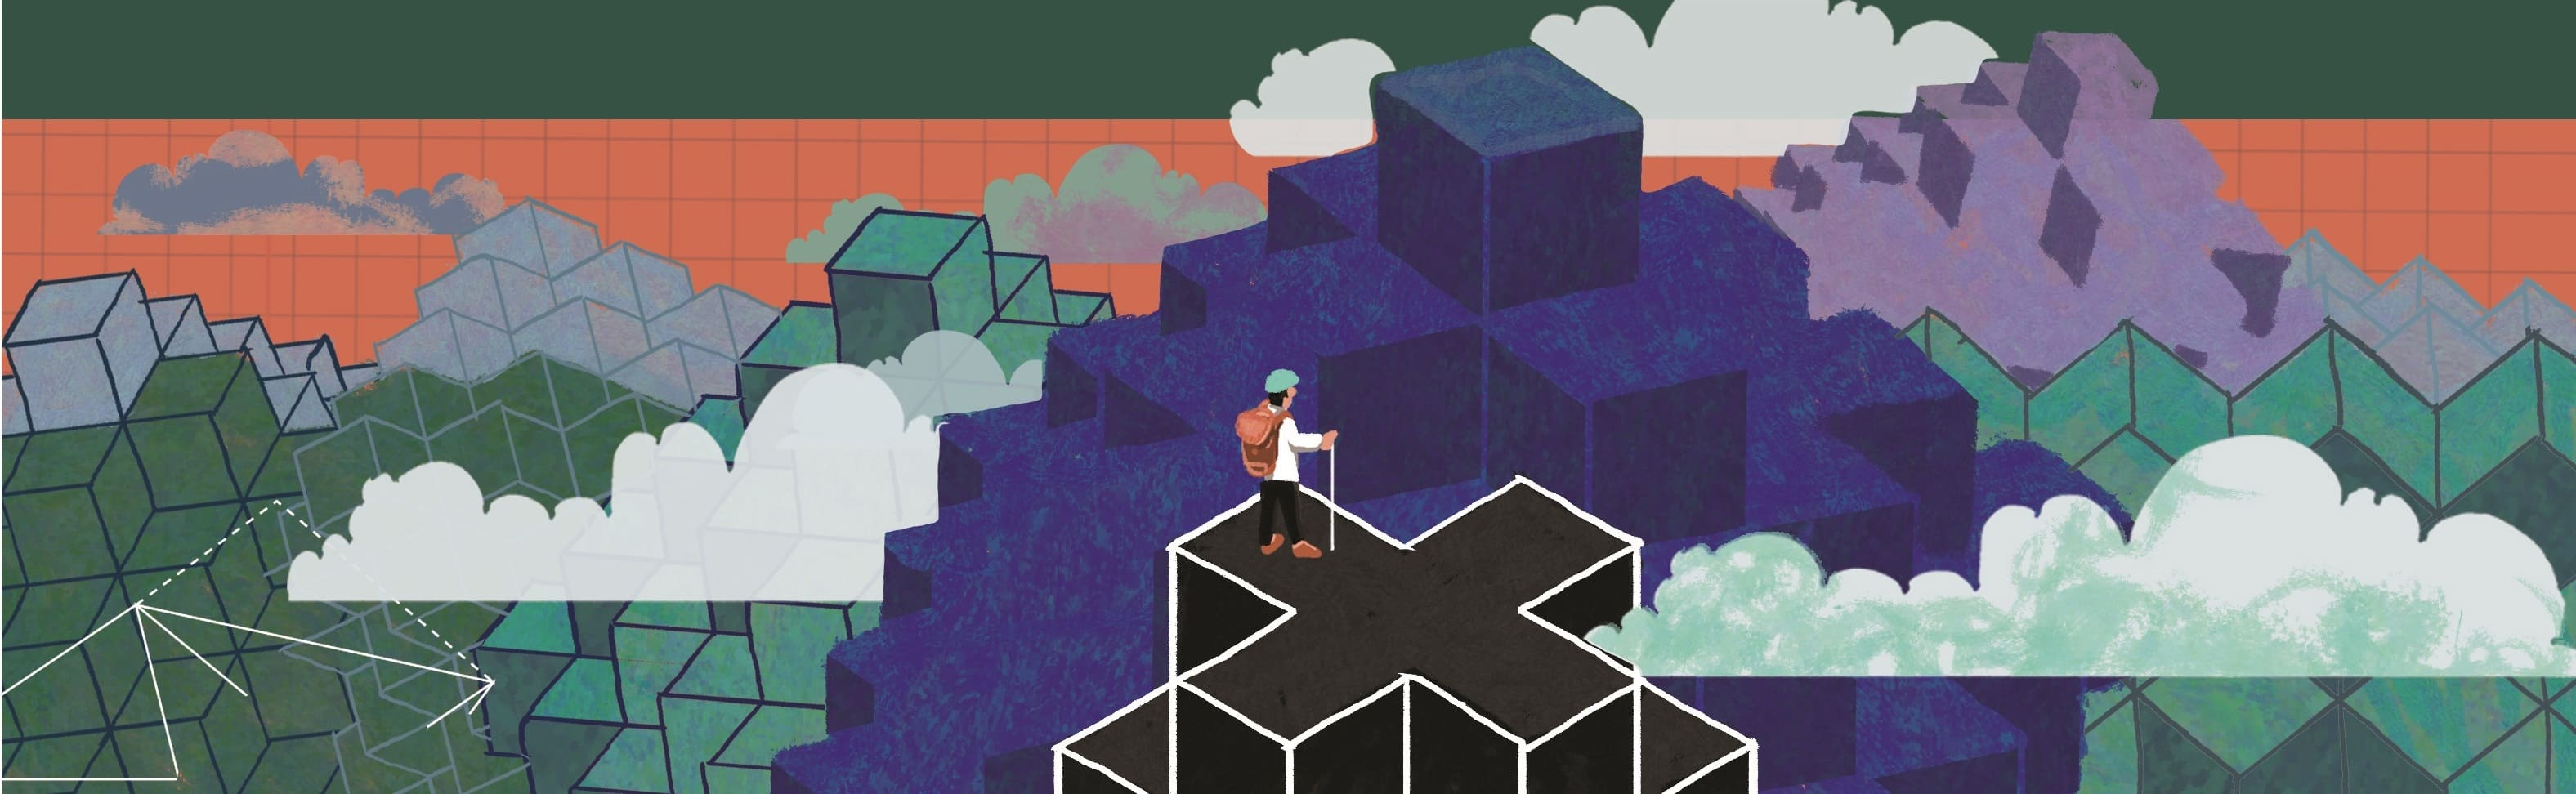
\includegraphics[width=19.3cm]{../thachthuctoanhoc/bannerthachthuc}}}
\centering
\vspace*{4cm}
\endgroup
\vspace*{-8pt}
\begin{tBox}
	\begin{itemize}[leftmargin = 13pt, itemsep = 1.0pt] 
		\item Mỗi bài toán đề xuất (kèm theo lời giải) cần được nêu rõ là bài sáng tác hay bài sưu tầm.
		%		\item Mỗi bài toán đề xuất (kèm theo lời giải) cần được nêu rõ là bài sáng tác hay bài sưu tầm (nếu là bài sưu tầm, cần ghi rõ nguồn).
		\item Bài giải cho mỗi bài toán cần được trình bày trong một file riêng hoặc
		một tờ giấy riêng.
		\item  Người đề xuất bài toán hoặc gửi bài giải cho các bài toán trong mục ``Thách thức kỳ này" cần ghi rõ họ, đệm, tên và nơi làm việc/học tập, số điện thoại liên hệ. Nếu là học sinh (hoặc sinh viên) cần ghi rõ là học sinh lớp mấy (hoặc sinh viên năm thứ mấy).
		\item Các bài toán trong mục Thách thức kỳ này hướng tới các độc giả là học sinh phổ thông; được phân chia thành các mức độ $B$, $A$, và được sắp xếp theo độ khó tăng dần, theo đánh giá chủ quan của Ban biên tập. Các bài toán mức độ $B$ không đòi hỏi các kiến thức vượt quá chương trình môn Toán cấp THCS; các bài toán mức độ $A$ không đòi hỏi các kiến thức vượt quá chương trình môn Toán cấp THPT.
		\item Cách thức gửi bài toán đề xuất hoặc lời giải: gửi file thu được bằng cách scan, ảnh chụp (rõ nét) của bản viết tay, hoặc được soạn thảo bằng các phần mềm Latex, Word tới \url{bbt@pi.edu.vn} hoặc gửi qua đường bưu điện tới Tòa soạn (xem địa chỉ tại bìa $2$).
		\item Hạn gửi lời giải cho các bài toán P$771$--P$780$: trước ngày $15/2/2024$.
	\end{itemize}
\end{tBox}
\begin{center}
	\vspace*{-5pt}
	\textbf{\color{thachthuctoanhoc}\color{thachthuctoanhoc}\color{thachthuctoanhoc}\color{thachthuctoanhoc}\color{thachthuctoanhoc}THÁCH THỨC KỲ NÀY}
	\vspace*{-5pt}
\end{center}
\begin{multicols}{2}
	\setlength{\abovedisplayskip}{4pt}
	\setlength{\belowdisplayskip}{4pt}
	{\color{thachthuctoanhoc}{\usefont{T5}{qag}{b}{n} P771.}}
	(Mức $B$) Để chuẩn bị cho việc biên soạn đề thi Olympic các môn khoa học năm $2024$, Ban tổ chức đã huy động một số giảng viên tham dự $10$ cuộc họp. Biết rằng, mỗi cuộc họp có đúng $20$ giảng viên tham dự và không có hai giảng viên nào cùng có mặt ở $2$ cuộc họp. Chứng minh rằng có ít nhất $63$ giảng viên được huy động để tham dự các cuộc họp.
	\begin{flushright}
		\textit{Duy Minh, Hà Nội}
	\end{flushright}
	{\color{thachthuctoanhoc}{\usefont{T5}{qag}{b}{n} P772.}}
	(Mức $B$) Cho $a$ là một số vô tỷ. Chứng minh rằng tồn tại số vô tỷ $b$ sao cho cho $a+b$ và $ab$ đều là các số vô tỷ.
	\begin{flushright}
		\textit{Vũ Hồng Sơn, Phú Thọ}
	\end{flushright}
	{\color{thachthuctoanhoc}{\usefont{T5}{qag}{b}{n} P773.}}
	(Mức $B$) Giải phương trình
	\begin{align*}
		2x^3-6x+5=0.
	\end{align*}
	\begin{flushright}
		\textit{Trần Văn Lâm, Thái Nguyên (st)}
	\end{flushright}
	{\color{thachthuctoanhoc}{\usefont{T5}{qag}{b}{n} P774.}}
	(Mức $B$) Cho $a, b, c$ là các số thực dương thỏa mãn $a b+b c+c a=3$. Chứng minh rằng
	\begin{align*}
		\dfrac{a^3}{b^2\!-\!b c\!+\!c^2}\!+\!\dfrac{b^3}{c^2\!-\!c a\!+\!a^2}\!+\!\dfrac{c^3}{a^2\!-\!a b\!+\!b^2} \!\geq\! 3.
	\end{align*}
	\begin{flushright}
		\textit{Nguyễn Việt Hùng, Hà Nội (st)}
	\end{flushright}
	{\color{thachthuctoanhoc}{\usefont{T5}{qag}{b}{n} P775.}}
	(Mức $B$) Cho tam giác $ABC$ và hai điểm $D, E$ lần lượt thuộc các cạnh $AC, AB$ sao cho
	\begin{align*}
		\angle{A B D}=\dfrac{1}{3} \angle{A B C} \text{và} \angle{A C E}=\dfrac{1}{3} \angle{A C B}.
	\end{align*}
	Gọi $K$ là giao điểm của $BD$ và $CE$.  Chứng minh rằng nếu $KD = KE$, thì tam giác $ABC$ hoặc là tam giác cân hoặc là tam giác vuông.
	\begin{figure}[H]
		\vspace*{-5pt}
		\centering
		\captionsetup{labelformat= empty, justification=centering}
		\begin{tikzpicture}[thachthuctoanhoc,scale=0.9]
			\draw  (4.,4.)-- (2.,0.);
			\draw  (2.,0.)-- (7.,0.);
			\draw  (7.,0.)-- (4.,4.);
			\draw  (2.,0.)-- (4.972074443691882,2.7039007417441585);
			\draw  (3.3115843535697493,2.6231687071394996)-- (7.,0.);
			\draw [fill=white] (4.,4.) circle (1.5pt);
			\draw (4.14,4.37) node {$A$};
			\draw [fill=white] (2.,0.) circle (1.5pt);
			\draw (1.68,-0.25) node {$B$};
			\draw [fill=white] (7.,0.) circle (1.5pt);
			\draw (7.14,0.37) node {$C$};
			\draw [fill=white] (4.972074443691882,2.7039007417441585) circle (1.5pt);
			\draw(5.12,3.03) node {$D$};
			\draw [fill=white] (3.3115843535697493,2.6231687071394996) circle (1.5pt);
			\draw (3.02,2.89) node {$E$};
			\draw [fill=white] (4.193734492595121,1.9957913013610344) circle (1.5pt);
			\draw(4.28,1.69) node {$K$};
		\end{tikzpicture}
		\vspace*{-10pt}
	\end{figure}
	\begin{flushright}
		\textit{Nguyễn Minh Hà, Hà Nội}
	\end{flushright}
	{\color{thachthuctoanhoc}{\usefont{T5}{qag}{b}{n} P776.}}
	(Mức $B$) Hai bạn Bảo và Hưng chơi một trò chơi luân phiên theo lượt, bạn Bảo đi trước. Trên một bảng $2 \times 6$, mỗi lượt người chơi điền một số nguyên dương chưa xuất hiện vào một ô trống. Khi tất cả các ô được điền, số lớn nhất trong mỗi hàng sẽ được tô màu đen. Bảo sẽ thắng nếu $2$ ô đen chung đỉnh, ngược lại, bạn Hưng là người chiến thắng. Hỏi ai là người có chiến lược chắc chắn thắng.
	\begin{flushright}
		\textit{Nguyễn Phúc Hưng, Đắk Nông}
	\end{flushright}
	{\color{thachthuctoanhoc}{\usefont{T5}{qag}{b}{n} P777.}}
	(Mức $A$) Tìm tất cả các hàm số \linebreak$f:{\mathbb R}^+\to {\mathbb R}^+$ thoả mãn 
	\begin{align*}
		f\left(x^2+ xf(y)+y\right)=2x+  f(y)
	\end{align*}
	với mọi $x,y\in{\mathbb R}^+$.
	\vskip 0.05cm
	(\textit{Ở đây, ${\mathbb R}^+$ là tập tất cả các số thực dương}.)
	\begin{flushright}
		\textit{Hồ Thanh Lai, Bình Định}
	\end{flushright}
	{\color{thachthuctoanhoc}{\usefont{T5}{qag}{b}{n} P778.}}
	(Mức $A$) Cho số nguyên tố $p$ thoả mãn $p\equiv 2\pmod3$. Tìm tất cả các cặp số tự nhiên $(x,y)$ thoả mãn 
	\begin{align*}
		x^3-y^3=19p\left(x^2+y^2\right).
	\end{align*}
	\begin{flushright}
		\textit{Kiều Đình Minh, Phú Thọ}
	\end{flushright}
	{\color{thachthuctoanhoc}{\usefont{T5}{qag}{b}{n} P779.}}
	(Mức $A$) Cho tứ giác lồi $ABCD$ có các cặp cạnh đối không song song. $AB$ cắt $CD$ tại $E$, $AD$ cắt $BC$ tại $F$ ($A$ nằm giữa $D$ và $F$, $C$ nằm giữa $D$ và $E$).  Gọi  $M, N$ tương  ứng là trung điểm $BD, AC$. $EM, EN$ lần lượt cắt $AC, BD$ tại $P, Q$. $FM, FN$ lần lượt cắt $AC, BD$ tại $R, S$. Chứng minh rằng, $PQ$ song song hoặc trùng với $RS$.
	\begin{figure}[H]
		\vspace*{-5pt}
		\centering
		\captionsetup{labelformat= empty, justification=centering}
		\definecolor{ffxfqq}{rgb}{1.,0.4980392156862745,0.}
		\definecolor{ffqqqq}{rgb}{1.,0.,0.}
		\definecolor{xfqqff}{rgb}{0.4980392156862745,0.,1.}
		\definecolor{ttffqq}{rgb}{0.2,1.,0.}
		\definecolor{qqccqq}{rgb}{0.,0.8,0.}
		\definecolor{uuuuuu}{rgb}{0.26666666666666666,0.26666666666666666,0.26666666666666666}
		\definecolor{qqqqff}{rgb}{0.,0.,1.}
		\definecolor{xdxdff}{rgb}{0.49019607843137253,0.49019607843137253,1.}
		\definecolor{ududff}{rgb}{0.30196078431372547,0.30196078431372547,1.}
		\begin{tikzpicture}[thachthuctoanhoc, node font=\small, scale=0.9]
			\draw [color=qqqqff] (3.5,2.96)-- (4.952681351616431,2.2543901179335926);
			\draw [color=qqqqff] (4.952681351616431,2.2543901179335926)-- (6.,0.);
			\draw [color=qqqqff] (6.,0.)-- (2.,0.);
			\draw [color=qqqqff] (2.,0.)-- (3.5,2.96);
			\draw [color=qqqqff] (3.5,2.96)-- (4.086867402040014,4.1180850066922945);
			\draw [color=qqqqff] (4.086867402040014,4.1180850066922945)-- (4.952681351616431,2.2543901179335926);
			\draw [color=qqqqff] (4.952681351616431,2.2543901179335926)-- (9.593929393664522,0.);
			\draw [color=qqqqff] (9.593929393664522,0.)-- (6.,0.);
			\draw [color=qqccqq] (2.,0.)-- (4.952681351616431,2.2543901179335926);
			\draw [color=ttffqq] (6.,0.)-- (3.5,2.96);
			\draw [color=xfqqff] (9.593929393664522,0.)-- (3.4763406758082156,1.1271950589667963);
			\draw [color=xfqqff] (4.170377292295862,1.657096224508167)-- (9.593929393664522,0.);
			\draw [color=ffqqqq] (4.086867402040014,4.1180850066922945)-- (4.75,1.48);
			\draw [color=ffqqqq] (4.086867402040014,4.1180850066922945)-- (3.4763406758082156,1.1271950589667963);
			\draw [color=ffxfqq] (5.337632505711885,0.7842431132371287)-- (4.170377292295862,1.657096224508167);
			\draw [color=ffxfqq] (4.6193213962686155,1.9998677704274923)-- (3.7822518887496273,2.6258137637204415);
			\draw [fill=white] (3.5,2.96) circle (1.5pt);
			\draw[color=ududff] (3.2423844117177434,3.2920617024009102) node {$A$};
			\draw [fill=white] (4.952681351616431,2.2543901179335926) circle (1.5pt);
			\draw[color=ududff] (5.079963400738184,2.589457971304859) node {$B$};
			\draw [fill=white] (6.,0.) circle (1.5pt);
			\draw[color=xdxdff] (5.962721934679377,-0.2569879136483735) node {$C$};
			\draw [fill=white] (2.,0.) circle (1.5pt);
			\draw[color=xdxdff] (1.9272543509482116,-0.34706531507094407) node {$D$};
			\draw [fill=white] (9.593929393664522,0.) circle (1.5pt);
			\draw[color=uuuuuu] (9.565817991582202,-0.2930188742174017) node {$E$};
			\draw [fill=white] (4.086867402040014,4.1180850066922945) circle (1.5pt);
			\draw[color=uuuuuu] (4.215220347081506,4.409021480040787) node {$F$};
			\draw [fill=white] (3.4763406758082156,1.1271950589667963) circle (1.5pt);
			\draw[color=uuuuuu] (3.4765856554164274,0.8599718639915027) node {$M$};
			\draw [fill=white] (4.75,1.48) circle (1.5pt);
			\draw[color=uuuuuu] (5.007901479600128,1.724714917648181) node {$N$};
			\draw [fill=white] (4.170377292295862,1.657096224508167) circle (1.5pt);
			\draw[color=uuuuuu] (3.9449881428137945,1.8328077993552658) node {$Q$};
			\draw [fill=white] (5.337632505711885,0.7842431132371287) circle (1.5pt);
			\draw[color=uuuuuu] (5.188056282445269,0.5356932188702483) node {$P$};
			\draw [fill=white] (3.7822518887496273,2.6258137637204415) circle (1.5pt);
			\draw[color=uuuuuu] (3.4765856554164274,2.6074734515893736) node {$R$};
			\draw [fill=white] (4.6193213962686155,1.9998677704274923) circle (1.5pt);
			\draw[color=uuuuuu] (4.683622834478873,2.3012102867526334) node {$S$};
		\end{tikzpicture}
		\vspace*{-10pt}
	\end{figure}
	\begin{flushright}
		\textit{Đỗ Thanh Sơn, Hà Nội}
	\end{flushright}
	{\color{thachthuctoanhoc}{\usefont{T5}{qag}{b}{n} P780.}}
	(Mức $A$) Ký hiệu $\pazocal{D}$ là tập tất cả các ước nguyên dương của $6^{2023}.$ Tìm số nguyên dương $k$ nhỏ nhất có tính chất, trong $k$ số bất kỳ thuộc $\pazocal{D}$, luôn tồn tại $3$ số có tích là lập phương của một số nguyên.
	\begin{flushright}
		\textit{Phạm Công Hoàn, Lai Châu}
	\end{flushright}
\end{multicols}
%\newpage
\centerline{{\large{\textbf{\color{thachthuctoanhoc}\color{thachthuctoanhoc}\color{thachthuctoanhoc}GIẢI BÀI KỲ TRƯỚC}}}}
\vspace*{-5pt}
\begin{multicols}{2}
	\setlength{\abovedisplayskip}{5pt}
	\setlength{\belowdisplayskip}{5pt}
	{\color{thachthuctoanhoc}{\usefont{T5}{qag}{b}{n} P741.}}
	(Mức $B$) Có $6$ tô phở giống hệt nhau được xếp thành hai chồng, như ở hình dưới đây: 
	\begin{figure}[H]
		\vspace*{-10pt}
		\centering
		\captionsetup{labelformat= empty, justification=centering}
		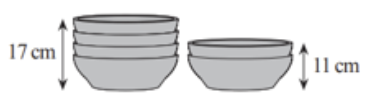
\includegraphics[width= 0.9\linewidth]{1}
		\vspace*{-5pt}
	\end{figure}
	Hỏi, nếu xếp cả $6$ tô phở thành một chồng, thì chiều cao của chồng đó là bao nhiêu?
	\vskip 0.05cm
	\textit{Lời giải} (\textit{của các bạn: Phạm Đức Minh, lớp $10$ Toán $2$, trường THPT chuyên Lê Hồng Phong, tỉnh Nam Định, và Võ Hải Yến, lớp $11$H, trường THPT chuyên Nguyễn Quang Diêu, tỉnh Đồng Tháp})\textbf{.}
	\vskip 0.05cm
	Từ giả thiết của bài toán, ta thấy, khi chồng thêm hai tô lên một chồng tô đã có thì chiều cao của chồng tô đã có đó sẽ tăng thêm
	\begin{align*}
		17 - 11 = 6 \text{ (cm)}.
	\end{align*}
	Vì vậy, do chồng gồm $4$ tô cao $17$ cm, nên khi chồng thêm hai tô lên chồng đó, ta sẽ có một chồng gồm $6$ tô, với chiều cao là:
	\begin{align*}
		17 + 6 = 23 \text{ (cm)}.
	\end{align*}
	\textit{Đáp số}: $23$ cm.
	\vskip 0.1cm
	\textbf{\color{thachthuctoanhoc}Bình luận và Nhận xét}
	\vskip 0.05cm	
	$\pmb{1.}$ Bài đã ra là một bài toán rất đơn giản, có thể sử dụng trong việc bồi dưỡng học sinh khá, giỏi Toán cấp Tiểu học.
	\vskip 0.05cm
	$\pmb{2.}$ Ngoại trừ hai bạn đã nêu tên ở phần Lời giải trên đây, hầu hết các bạn còn lại, trong số các bạn đã gửi lời giải tới Tạp chí, đều giải bài đã ra bằng cách lập hệ phương trình. Rất tiếc, trong số này, có một bạn có lời giải sai, do đã lập sai hệ phương trình.
	\begin{flushright}
		\textbf{\color{thachthuctoanhoc}Hà Thanh}
	\end{flushright}
	{\color{thachthuctoanhoc}{\usefont{T5}{qag}{b}{n} P742.}}
	(Mức $B$) Cho $10$ số hữu tỷ $a_1,\ldots,a_{10}$ khác $0$ và thoả mãn
	\vskip 0.05cm
	$i/$ $a_1+\cdots+a_8=a_1a_2\cdots a_8$. 
	\vskip 0.05cm
	$ii/$ $a_1+\cdots+a_9=a_1a_2\cdots a_9$. 
	\vskip 0.05cm
	$iii/$ $a_1+\cdots+a_{10}=a_1a_2\cdots a_{10}$. 
	\vskip 0.05cm
	Chứng minh rằng, $\dfrac{4-3a_{10}}{a_{10}}$ là bình phương của một số hữu tỷ.
	\vskip 0.05cm
	\textbf{\color{thachthuctoanhoc}Lời giải} (\textit{dựa theo đa số lời giải Tạp chí đã nhận được từ bạn đọc})\textbf{\color{thachthuctoanhoc}.}
	\vskip 0.05cm
	Từ $i/$ và $ii/$, suy ra
	\begin{align*}
		{a_9} = {a_1}{a_2} \cdots {a_8} \cdot \left( {{a_9} - 1} \right). \tag{$1$}
	\end{align*}
	Từ $ii/$ và $iii/$, suy ra
	\begin{align*}
		{a_{10}} = {a_1}{a_2} \cdots {a_8} \cdot {a_9} \cdot \left( {{a_{10}} - 1} \right)
	\end{align*}
	Do $a_i \ne 0$ với mọi $i = \overline{1,9}$  nên từ ($1$) suy ra, $a_9 \ne 1$.  Vì thế, chia ($2$) cho ($1$), vế theo vế, ta được:
	\begin{align*}
		\frac{{{a_{10}}}}{{{a_9}}} = \frac{{{a_9} \cdot \left( {{a_{10}} - 1} \right)}}{{{a_9} - 1}};
	\end{align*}
	do đó
	\begin{align*}
		{a_{10}}\left( {a_9^2 - {a_9} + 1} \right) = a_9^2.
	\end{align*}
	Suy ra
	\begin{align*}
		{a_{10}} = \frac{{a_9^2}}{{a_9^2 - {a_9} + 1}};
	\end{align*}
	vì vậy
	\begin{align*}
		\frac{{4 - 3{a_{10}}}}{{{a_{10}}}} &= \frac{4}{{{a_{10}}}} - 3 = \frac{{4\left( {a_9^2 - {a_9} + 1} \right)}}{{a_9^2}} - 3 \\
		&= \frac{{a_9^2 - 4{a_9} + 4}}{{a_9^2}} \\
		&= {\left( {\frac{{{a_9} - 2}}{{{a_9}}}} \right)^2}.
	\end{align*}
	Do $a_9$ là số hữu tỷ, nên $\dfrac{a_9 - 2}{a_9}$ cũng là số hửu tỷ. Vì vậy, ($3$) cho ta điều phải chứng minh theo yêu cầu đề bài.
	\vskip 0.05cm
	\textbf{\color{thachthuctoanhoc}Bình luận và Nhận xét}
	\vskip 0.05cm
	Tất cả lời giải Tạp chí đã nhận được từ bạn đọc đều là lời giải đúng.
	\begin{flushright}
		\textbf{\color{thachthuctoanhoc}Lưu Thị Thanh Hà}
	\end{flushright}
	{\color{thachthuctoanhoc}{\usefont{T5}{qag}{b}{n} P743.}}
	(Mức $B$) Cho tam giác $A B C$ không cân, có đường cao $A H$ và phân giác trong $A D$. Tiếp tuyến tại $A$ của đường tròn ngoại tiếp tam giác đó cắt đường thẳng $B C$ tại $M$. Gọi $E$ là hình chiếu vuông góc của $B$ trên đường phân giác ngoài của góc $A$. Chứng minh rằng, các đường thẳng $C E, A D$ cắt nhau tại một điểm nằm trên đường tròn ngoại tiếp tam giác $A M H.$
	\vskip 0.05cm
	\textbf{\color{thachthuctoanhoc}Lời giải} (\textit{của người chấm bài})\textbf{\color{thachthuctoanhoc}.}
	\vskip 0.1cm
	Ký hiệu $(O)$ là đường tròn ngoại tiếp tam giác $ABC$.
	\vskip 0.05cm
	Gọi $I$ là giao điểm của $CA$ và $BE$; $J$ là giao điểm của $CE$ và $AD$.
	\vskip 0.05cm
	Do là phân giác ngoài của góc $CAB$, nên $AE$ là phân giác trong của góc $BAI$. Mà $BI \bot AE$ nên $I$ đối xứng với $B$ qua $AE$; do đó, $E$ là trung điểm của $BI$. \hfill ($1$)
	\vskip 0.05cm 
	Do $AD$ và $AE$ tương ứng là phân giác trong và phân giác ngoài của góc $BAC$, nên $AD \bot AE$. Suy ra, $AD \parallel IB$ (vì cùng vuông góc với $AE$). \hfill ($2$)
	\vskip 0.05cm
	Do $IA$, $BD$, $EJ$ đồng quy tại $C$, nên từ ($2$) và ($1$) suy ra, $J$ là trung điểm của $AD$. \hfill ($3$)
	\vskip 0.05cm
	Tiếp theo, ta có:
	\begin{figure}[H]
		\vspace*{-5pt}
		\centering
		\captionsetup{labelformat= empty, justification=centering}
		\definecolor{qqwuqq}{rgb}{0.,0.39215686274509803,0.}
		\definecolor{ffqqqq}{rgb}{1.,0.,0.}
		\definecolor{uuuuuu}{rgb}{0.26666666666666666,0.26666666666666666,0.26666666666666666}
		\definecolor{qqqqff}{rgb}{0.,0.,1.}
		\begin{tikzpicture}[thachthuctoanhoc, scale=0.45]
			\draw[pattern color=qqwuqq,fill=qqwuqq,fill opacity=0.10000000149011612] (-0.1577556526664092,2.6482609129258585) -- (0.17545239323611356,2.754002664369888) -- (0.06971064179208414,3.0872107102724105) -- (-0.26349740411043865,2.981468958828381) -- cycle; 
			\draw[pattern color=qqwuqq,fill=qqwuqq,fill opacity=0.10000000149011612] (2.486791954097477,3.8542582485559707) -- (2.5925337055415065,3.5210502026534476) -- (2.925741751444029,3.6267919540974773) -- (2.82,3.96) -- cycle; 
			\draw[pattern color=qqwuqq,fill=qqwuqq,fill opacity=0.10000000149011612] (2.82,-0.6504160760952692) -- (2.470416076095269,-0.6504160760952691) -- (2.470416076095269,-1.) -- (2.82,-1.) -- cycle; 
			\draw[pattern color=ffqqqq,fill=white,fill opacity=0.10000000149011612] (3.501272688351068,1.8132080459025233) -- (3.1680646424485452,1.7074662944584937) -- (3.2738063938925746,1.3742582485559711) -- (3.607014439795097,1.48) -- cycle; 
			\draw [shift={(2.82,3.96)},pattern color=qqwuqq,fill=qqwuqq,fill opacity=0.10000000149011612] (0,0) -- (-110.14987901844857:0.9887726527473487) arc (-110.14987901844857:-72.39344899560092:0.9887726527473487) -- cycle;
			\draw [shift={(2.82,3.96)},pattern color=qqwuqq,fill=qqwuqq,fill opacity=0.10000000149011612] (0,0) -- (-72.39344899560092:0.7415794895605115) arc (-72.39344899560092:-34.63701897275325:0.7415794895605115) -- cycle;
			\draw [shift={(10.,-1.)},pattern color=qqwuqq,fill=qqwuqq,fill opacity=0.10000000149011612] (0,0) -- (145.36298102724675:0.7415794895605115) arc (145.36298102724675:180.:0.7415794895605115) -- cycle;
			\draw [shift={(2.82,3.96)},pattern color=qqwuqq,fill=qqwuqq,fill opacity=0.10000000149011612] (0,0) -- (-144.78689799120178:0.7415794895605115) arc (-144.78689799120178:-110.14987901844857:0.7415794895605115) -- cycle;
			\draw  (2.82,3.96)-- (1.,-1.);
			\draw  (10.,-1.)-- (2.82,3.96);
			\draw  (5.5,0.16270161290322593) circle (4.647781733326959cm);
			\draw [dash pattern=on 6pt off 6pt,color=ffqqqq] (-0.6939179104477596,1.48) circle (4.3009323502428565cm);
			\draw (2.5344197037187493,5.4991055179118128) node[anchor=north west] {$A$};
			\draw (0.2074357655866845,-1.138262068164937) node[anchor=north west] {$B$};
			\draw (9.999653231961231,-0.6943875741791262) node[anchor=north west] {$C$};
			\draw (4.388368427620028,-1.1943875741791262) node[anchor=north west] {$D$};
			\draw (2.5838583363561165,-1.1910689049781) node[anchor=north west] {$H$};
			\draw (-4.881375191886366,-1.1910689049781) node[anchor=north west] {$M$};
			\draw  (2.82,-1.)-- (2.82,3.96);
			\draw  (-4.207835820895519,-1.)-- (2.82,3.96);
			\draw [color=qqqqff] (1.,-1.)-- (-0.26349740411043865,2.981468958828381);
			\draw [color=qqqqff] (0.28839489530837914,0.8746228760576574) -- (0.5004471972316128,0.9419165146082121);
			\draw [color=qqqqff] (0.2622251469831636,0.9570876601389144) -- (0.47427744890639734,1.0243812986894691);
			\draw [color=qqqqff] (0.23605539865794814,1.0395524442201716) -- (0.4481077005811818,1.1068460827707263);
			\draw  (-0.26349740411043865,2.981468958828381)-- (10.,-1.);
			\draw (5.5007376619607955,0.46742029279900826) node[anchor=north west] {$O$};
			\draw (-1.5757232135343386,3.755089363183942) node[anchor=north west] {$E$};
			\draw (3.622069621740833,2.472110677442356) node[anchor=north west] {$J$};
			\draw  (3.607014439795097,1.48)-- (2.82,-1.);
			\draw  (-4.207835820895519,-1.)-- (3.607014439795097,1.48);
			\draw  (2.82,3.96)-- (-1.526994808220878,6.962937917656762);
			\draw (-2.3934498919055,7.809057239448071) node[anchor=north west] {$I$};
			\draw [color=qqqqff] (-0.26349740411043865,2.981468958828381)-- (-1.526994808220878,6.962937917656762);
			\draw [color=qqqqff] (-0.9751025088020592,4.856091834886038) -- (-0.7630502068788255,4.923385473436592);
			\draw [color=qqqqff] (-1.0012722571272747,4.938556618967295) -- (-0.789219955204041,5.005850257517849);
			\draw [color=qqqqff] (-1.0274420054524902,5.021021403048553) -- (-0.8153897035292564,5.088315041599107);
			\draw [color=qqqqff] (3.607014439795097,1.48)-- (4.394028879590194,-1.);
			\draw [color=qqqqff] (4.0934629364916555,0.3148792113159061) -- (3.8814106345684216,0.24758557276535137);
			\draw [color=qqqqff] (4.11963268481687,0.23241442723464906) -- (3.907580382893636,0.16512078868409433);
			\draw [color=qqqqff] (3.607014439795097,1.48)-- (2.82,3.96);
			\draw [color=qqqqff] (3.12056594309854,2.645120788684094) -- (3.332618245021774,2.7124144272346484);
			\draw [color=qqqqff] (3.094396194773325,2.7275855727653506) -- (3.306448496696559,2.7948792113159056);
			\draw  (-0.26349740411043865,2.981468958828381)-- (2.82,3.96);
			\draw  (-4.207835820895519,-1.)-- (10.,-1.);
			\draw [shift={(2.82,3.96)},color=qqwuqq] (-110.14987901844857:0.9887726527473487) arc (-110.14987901844857:-72.39344899560092:0.9887726527473487);
			\draw [shift={(2.82,3.96)},color=qqwuqq] (-110.14987901844857:0.8651760711539301) arc (-110.14987901844857:-72.39344899560092:0.8651760711539301);
			\draw [shift={(2.82,3.96)},color=qqwuqq] (-72.39344899560092:0.7415794895605115) arc (-72.39344899560092:-34.63701897275325:0.7415794895605115);
			\draw [shift={(2.82,3.96)},color=qqwuqq] (-72.39344899560092:0.6179829079670929) arc (-72.39344899560092:-34.63701897275325:0.6179829079670929);
			\begin{scriptsize}
				\draw [fill=white] (2.82,3.96) circle (1.5pt);
				\draw [fill=white] (1.,-1.) circle (1.5pt);
				\draw [fill=white] (10.,-1.) circle (1.5pt);
				\draw [fill=white] (-4.207835820895519,-1.) circle (1.5pt);
				\draw [fill=white] (-0.26349740411043865,2.981468958828381) circle (1.5pt);
				\draw [fill=white] (3.607014439795097,1.48) circle (1.5pt);
				\draw [fill=white] (2.82,-1.) circle (1.5pt);
				\draw [fill=white] (4.394028879590194,-1.) circle (1.5pt);
				\draw [fill=white] (5.5,0.16270161290322593) circle (1.5pt);
				\draw [fill=white] (-1.526994808220878,6.962937917656762) circle (1.5pt);
			\end{scriptsize}
		\end{tikzpicture}
		\caption{\small\textit{\color{thachthuctoanhoc}Hình $1$. $(AB < AC)$}}
		\vspace*{-10pt}
	\end{figure}
	-- Nếu $AB < AC$ (xem Hình $1$) thì tia $AB$ nằm giữa hai tia $AM$ và $AD$. Do đó
	\begin{align*}
		&\angle MAB = \angle ACB \text{ (vì $MA$ tiếp xúc $(O)$ tại $A$),}\\
		&\angle MAD = \angle MAB + \angle BAD.
	\end{align*}
	Từ đó, với lưu ý $AD$ là phân giác trong của góc $BAC$, suy ra
	\begin{align*}
		\angle MAD = \angle ACB + \angle CAD = \angle ADM.
	\end{align*}
	\begin{figure}[H]
		\vspace*{-10pt}
		\centering
		\captionsetup{labelformat= empty, justification=centering}
		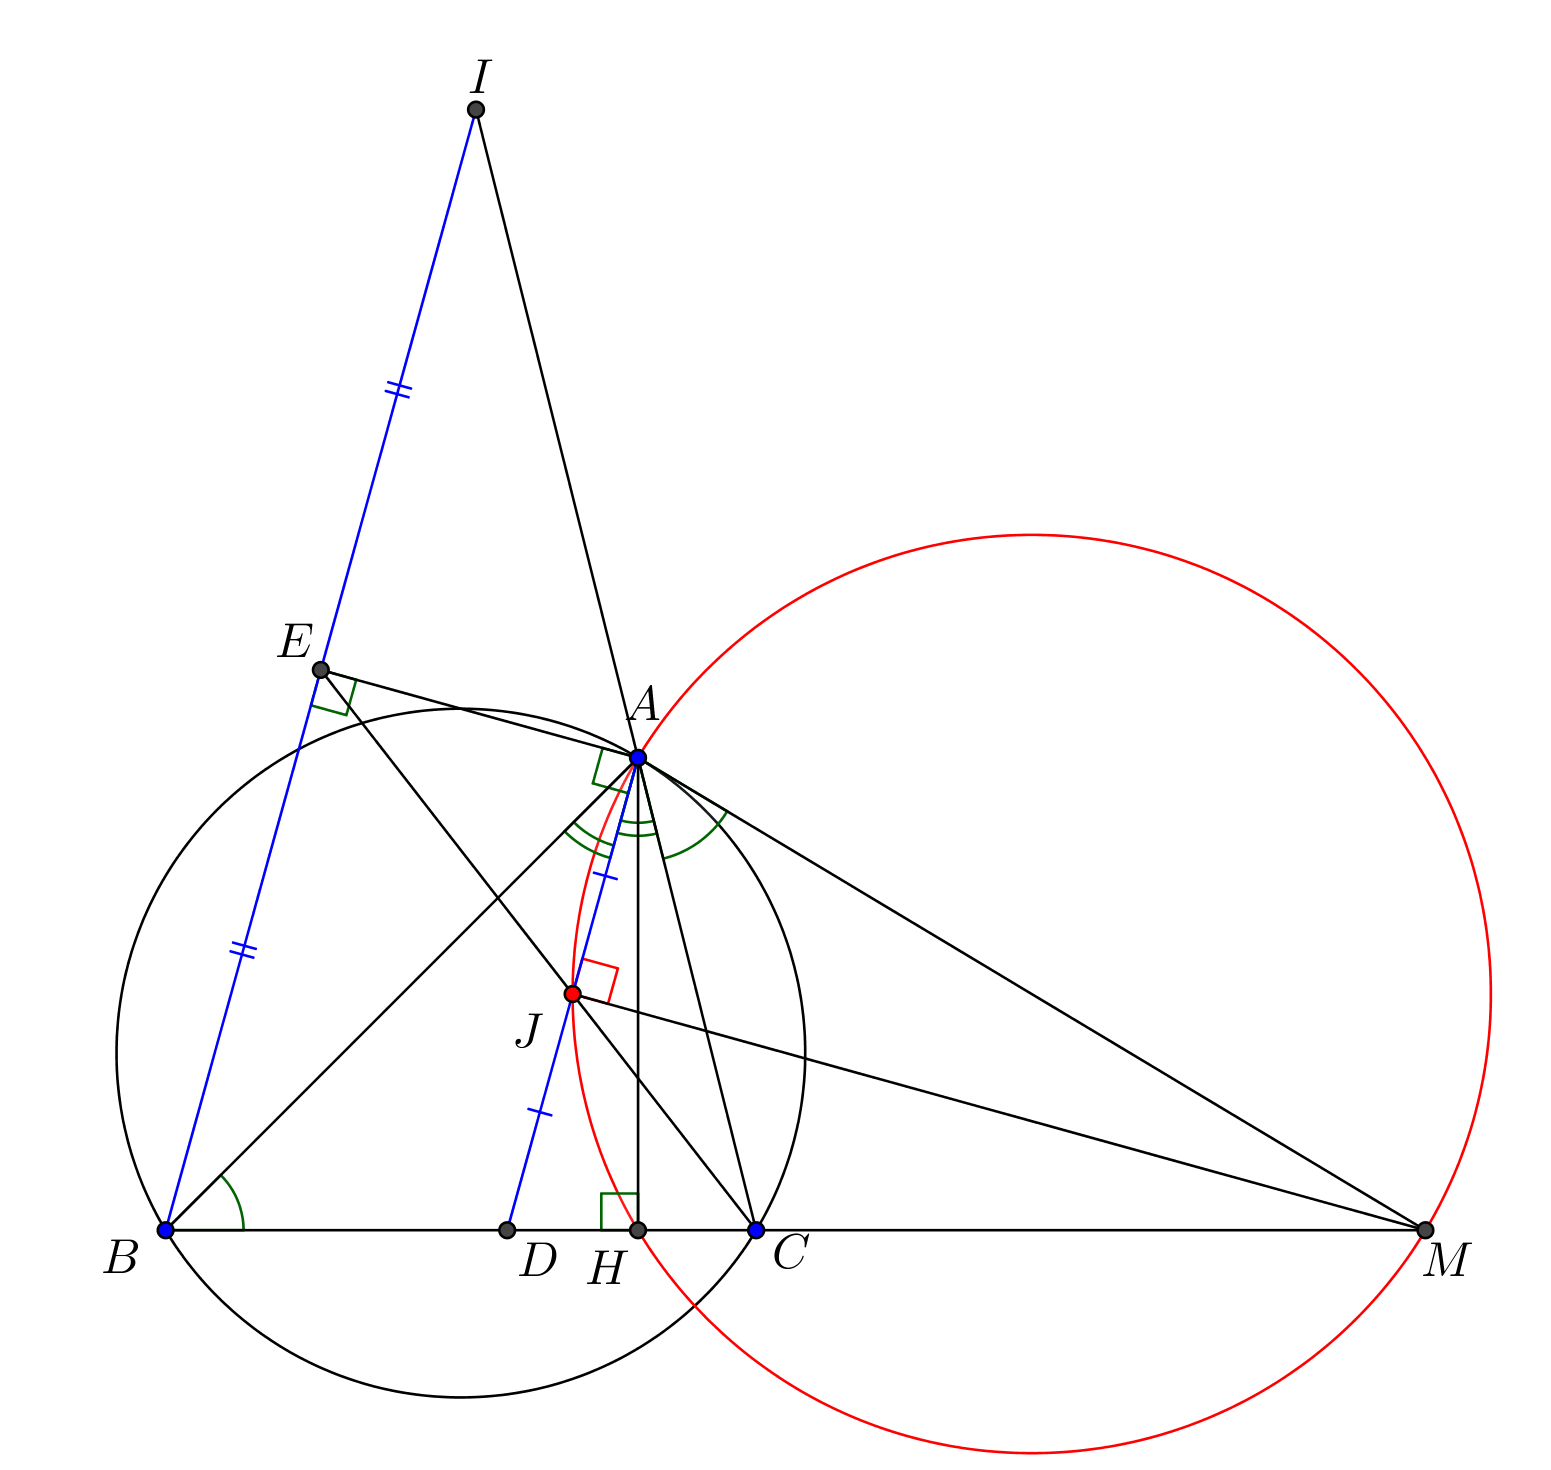
\includegraphics[width= 1\linewidth]{P743-Fig1}
		\caption{\small\textit{\color{thachthuctoanhoc}Hình $2$. $(AB > AC)$}}
		\vspace*{-10pt}
	\end{figure}
	-- Nếu $AB > AC$ (xem Hình $2$) thì tia $AC$ nằm giữa hai tia $AM$ và $AD$. Do đó
	\begin{align*}
		&\angle MAC = \angle ABC \text{ (vì $MA$ tiếp xúc $(O)$ tại $A$),}\\
		&\angle MAD = \angle MAC + \angle CAD.
	\end{align*}
	Từ đó, với lưu ý $AD$ là phân giác trong của góc $CAB$, suy ra
	\begin{align*}
		\angle MAD = \angle ABC + \angle BAD = \angle ADM.
	\end{align*}
	Như vậy, với $ABC$ là tam giác không cân, ta có $AMD$ là tam giác cân tại $M$. Từ đây và ($3$), suy ra $MJ \bot AJ$; do đó,
	\begin{align*}
		&\angle AJM = 90^\circ = \angle AHM \\
		&\text{ (vì $AH \bot BC$, theo giả thiết).}
	\end{align*}
	Vì vậy, bốn điểm $A$, $J$, $H$, $M$ cùng nằm trên một đường tròn; hay, giao điểm của $CE$ và $AD$ nằm trên đường tròn ngoại tiếp tam giác $AMH$. Ta có điều phải chứng minh theo yêu cầu đề bài.
	\vskip 0.05cm
	\textbf{\color{thachthuctoanhoc}Bình luận và Nhận xét}
	\vskip 0.05cm
	$\pmb{1.}$ Do $AMH$ là tam giác vuông tại $H$ (theo giả thiết), nên đường tròn ngoại tiếp tam giác đó là đường tròn đường kính $AM$. Vì thế, kết luận của đề bài tương đương với $MJ \bot AJ$, trong đó, $J$ là giao điểm của $CE$ và $AD$. Điều này gợi ý việc tìm hiểu tam giác $AMD$.
	\vskip 0.05cm
	Dễ dàng nhận ra, tam giác $AMD$ cân tại $M$. Vì thế, $MJ \bot AJ$ tương đương với $J$ là trung điểm của $AD$.
	\vskip 0.05cm
	Để ý rằng $DA \parallel BE$, sẽ thấy ngay, $J$ là trung điểm của $AD$ tương đương với $E$ là trung điểm của $BI$, trong đó, $I$ là giao điểm của $CA$ và $BE$.
	\vskip 0.05cm
	Lời giải trên đây là ``sản phẩm" của những nhận xét và suy diễn đơn giản nêu trên.
	\vskip 0.05cm
	$\pmb{2.}$ Những suy diễn đã nêu ở $1$. cho thấy, bài đã ra là một bài toán nhẹ nhàng, giúp người giải bài hình thành và rèn luyện tư duy hình học trong sáng.
	\vskip 0.05cm
	$\pmb{3.}$ Một số bạn đọc đã dùng những công cụ quá mạnh (hàng điểm điều hòa, chùm điều hòa, phương tích của một điểm đối với một đường tròn, \ldots) để giải bài đã ra.
	\vskip 0.05cm
	$\pmb{4.}$ Tất cả lời giải Tạp chí đã nhận được từ bạn đọc, rất tiếc, đều là lời giải chưa đúng, do người giải bài chưa xét hết các cấu hình có thể, hoặc \textit{ngộ nhận} rằng, ``không mất tổng quát, có thể giả sử $AB < AC$".
	\begin{flushright}
		\textbf{\color{thachthuctoanhoc}Hạ Vũ Anh}
	\end{flushright}
	{\color{thachthuctoanhoc}{\usefont{T5}{qag}{b}{n} P744.}}
	(Mức $B$) Giải hệ phương trình 
	\begin{align*}
		\begin{cases}
			x+y=2+\sqrt{xy(xy-3)}&\\
			xy(x-y)=2(2-x).
		\end{cases}
	\end{align*}
	\textbf{\color{thachthuctoanhoc}Lời giải} (\textit{dựa theo cách giải của bạn Nguyễn Chánh Thiện, lớp $9/12$, trường THCS Lê Quý Đôn, Quận $3$, Tp. Hồ Chí Minh})\textbf{\color{thachthuctoanhoc}.}
	\vskip 0.05cm
	Điều kiện xác định của hệ phương trình:
	\begin{align*}
		\left[ \begin{array}{l}
			xy \le 0\\
			xy \ge 3.
		\end{array} \right. \tag{$1$}
	\end{align*}
	Từ phương trình thứ nhất của hệ, dễ thấy, nếu ($x, y)$ là nghiệm của hệ đã cho thì \linebreak $x + y \ge  2$.   \hfill  ($2$)
	\vskip 0.05cm
	Vì vậy, $(x, y)$ là nghiệm của hệ đã cho chỉ khi $x, y$ thỏa mãn đồng thời ($1$) và ($2$).
	\vskip 0.05cm
	Xét $(x, y)$ mà $x, y$ là các số thực thỏa mãn đồng thời ($1$) và ($2$).
	\vskip 0.05cm
	Khi đó, hệ đã cho tương đương với hệ:
	\begin{align*}
		\begin{cases}
			{\left( {x + y - 2} \right)^2} = xy\left( {xy - 3} \right)\\
			xy\left( {x - y} \right) = 2\left( {2 - x} \right).
		\end{cases} \tag{$\text{I}$}
	\end{align*}
	Ta có:
	\vskip 0.05cm
	\scalebox{0.9}{\parbox{1\linewidth}{\begin{align*}
		&\text{(I)}\\
		\Leftrightarrow &\begin{cases}
			{\left( {x \!+\! y} \right)^2} \!-\! 4\left( {x \!+\! y} \right) \!-\! \left( {{x^2}{y^2} \!-\! 3xy \!-\! 4} \right) \!=\! 0\\
			xy\left( {x - y} \right) + \left( {x - y} \right) = 4 - \left( {x + y} \right)
		\end{cases}\\
	\Leftrightarrow & \begin{cases}
		\left( {x + y} \right)\left( {x + y - 4} \right) - \left( {xy + 1} \right)\left( {xy - 4} \right) = 0\\
		\left( {x - y} \right)\left( {xy + 1} \right) = 4 - \left( {x + y} \right)
	\end{cases}\\
	\Leftrightarrow & \begin{cases}
		\left( {x \!+\! y} \right)\left( {y \!-\! x} \right)\left( {xy \!+\! 1} \right) \!-\! \left( {xy \!+\! 1} \right)\left( {xy \!-\! 4} \right) \!=\! 0\\
		x + y - 4 = \left( {y - x} \right)\left( {xy + 1} \right)
	\end{cases}\\
	\Leftrightarrow & \begin{cases}
		\left( {xy + 1} \right)\left( {{x^2} - {y^2} + xy - 4} \right) = 0\\
		x + y - 4 = \left( {y - x} \right)\left( {xy + 1} \right)
	\end{cases}\\
	\Leftrightarrow & \left[\begin{array}{l}
		\begin{cases}
			xy =  - 1\\
			x + y = 4
		\end{cases} \quad\quad\quad\quad\quad\quad\quad\quad\quad\quad\!\!\text{(II)}\\
		\begin{cases}
			{x^2}\, - {y^2}\, + xy - 4 = 0\\
			x + y - 4 = \left( {y - x} \right)\left( {xy + 1} \right).
		\end{cases}	\quad\quad\text{(III)}
	\end{array} \right.
	\end{align*}}}
	\vskip 0.05cm
	Theo định lý Vi--et đảo cho phương trình bậc hai, $(x, y)$ là nghiệm của hệ ($\text{II}$) khi và chỉ khi $x, y$ là hai nghiệm của phương trình (ẩn $t$):
	\begin{align*}
		t^2 - 4t - 1 = 0.
	\end{align*}
	Vì thế, từ kết quả giải phương trình vừa nêu trên, ta được:
	\begin{align*}
		\text{II} \Leftrightarrow \left[ \begin{array}{l}
			\left( {x,y} \right) = \left( {2 - \sqrt 5 ,2 + \sqrt 5 } \right)\\
			\left( {x,y} \right) = \left( {2 + \sqrt 5 ,2 - \sqrt 5 } \right).
		\end{array} \right.
	\end{align*}  
	Hiển nhiên, hai cặp số $(x, y)$ vừa nêu trên thỏa mãn đồng thời ($1$) và ($2$). Vì thế, chúng là các nghiệm của hệ phương trình trong đề bài.
	\vskip 0.05cm
	Xét hệ ($\text{III}$); ta có:
	\vskip 0.05cm
	\scalebox{0.9}{\parbox{1\linewidth}{\begin{align*}
		&\text{(III)}\\
		\Leftrightarrow& \begin{cases}
			y\left( {y - x} \right) = {x^2} - 4\\
			xy\left( {y - x} \right) = 2x - 4
		\end{cases}\\
	\Leftrightarrow & \begin{cases}
		y\left( {y - x} \right) = {x^2} - 4\\
		x\left( {{x^2} - 4} \right) = 2x - 4
	\end{cases}\\
	\Leftrightarrow & \begin{cases}
		y\left( {y - x} \right) = {x^2} - 4\\
		\left( {x - 2} \right)\left( {{x^2} + 2x - 2} \right) = 0
	\end{cases} \\
	\Leftrightarrow & \left[ \begin{array}{l}
		\begin{cases}
			x = 2\\
			y\left( {y - 2} \right) = 0
		\end{cases} \quad\quad\quad\quad\quad\quad\quad\quad\!\!\text{(IV)}\\
		\begin{cases}
			{x^2} + 2x - 2 = 0\\
			y\left( {y - x} \right) = {x^2} - 4.
		\end{cases}\quad\quad\quad\quad\quad\quad\text{(V)}
	\end{array} \right.
	\end{align*}}}
	\vskip 0.05cm
	Giải hệ ($\text{IV}$), ta được $(x, y)$ = $(2, 0)$ và $(x, y) = (2, 2)$. Dễ thấy, cả hai cặp số vừa nêu đều thỏa mãn đồng thời ($1$) và ($2$). Vì thế, chúng là các nghiệm của hệ phương trình trong đề bài.
	\vskip 0.05cm
	Xét hệ ($\text{V}$); ta có:
	\begin{align*}
		\text{V} \Leftrightarrow \left\{ \begin{array}{l}
			{x^2} + 2x - 2 = 0\left( 3 \right)\\
			y\left( {y - x} \right) =  - 2\left( {x + 1} \right).\left( 4 \right)
		\end{array} \right.
	\end{align*}
	Giải phương trình ($3$), ta được $x = -1 - \sqrt{3}$  và $x = -1 + \sqrt{3}$.
	\vskip 0.05cm 
	-- Thế $x = -1 - \sqrt{3}$  vào ($4$), ta được
	\begin{align*}
		{y^2} + \left( {1 + \sqrt 3 } \right)y - 2\sqrt 3  = 0.
	\end{align*}
	Giải phương trình vừa nêu trên, ta được
	\begin{align*}
		&y = {y_1} = \frac{{ - \left( {1 + \sqrt 3 } \right) - \sqrt {4 + 10\sqrt 3 } }}{2} \\
		\text{và } &y = {y_2} = \frac{{ - \left( {1 + \sqrt 3 } \right) + \sqrt {4 + 10\sqrt 3 } }}{2}
	\end{align*}
	Với $\left( {x,y} \right) = \left( { - 1 - \sqrt 3 ,{y_1}} \right),$  hiển nhiên có $x + y < 0 < 2$. \hfill ($5$)
	\vskip 0.05cm
	Xét $\left( {x,y} \right) = \left( { - 1 - \sqrt 3 ,{y_2}} \right).$ Do
	\begin{align*}
		\sqrt {4 + 10\sqrt 3 }  < \sqrt {24}  < 5 < 4 + 3\left( {1 + \sqrt 3 } \right),
	\end{align*}
	nên  ${y_2} < 2 + \left( {1 + \sqrt 3 } \right);$ suy ra
	\begin{align*}
		x + y =  - \left( {1 + \sqrt 3 } \right) + {y_2} < 2. \tag{$6$}
	\end{align*}
	($5$) và ($6$) cho thấy, cả hai cặp số $\left( {x,y} \right) = \left( { - 1 - \sqrt 3 ,{y_1}} \right)$  và $\left( {x,y} \right) = \left( { - 1 - \sqrt 3 ,{y_2}} \right)$  đều không thỏa mãn ($2$). Vì thế, chúng không là nghiệm của hệ phương trình trong đề bài.
	\vskip 0.05cm
	-- Thế  $x =  - 1 + \sqrt 3 $ vào ($4$), ta được:
	\begin{align*}
		{y^2} + \left( {1 - \sqrt 3 } \right)y + 2\sqrt 3  = 0.
	\end{align*}
	Phương trình vừa nêu trên có
	\begin{align*}
		\Delta  = 4 - 10\sqrt 3  < 0,
	\end{align*}
	nên nó vô nghiệm.
	\vskip 0.05cm
	Vậy, tóm lại, hệ phương trình trong đề bài có tất cả bốn nghiệm, là:
	\begin{align*}
		&\left( {x,y} \right) = \left( {2 - \sqrt 5 ,2 + \sqrt 5 } \right),\\
		&\left( {x,y} \right) = \left( {2 + \sqrt 5 ,2 - \sqrt 5 } \right),\\
		&\left( {x,y} \right) = \left( {2,0} \right) \text{ và } \left( {x,y} \right) = \left( {2,2} \right).
	\end{align*}
	\textbf{\color{thachthuctoanhoc}Bình luận và Nhận xét}
	\vskip 0.05cm
	Trong số các lời giải Tạp chí đã nhận được từ bạn đọc, rất tiếc, có một lời giải sai, do người giải bài đã mắc lỗi kiến thức cơ bản, khi đồng nhất ``hệ số" trong quá trình biến đổi các phương trình của hệ phương trình đã cho.
	\begin{flushright}
		\textbf{\color{thachthuctoanhoc}Hoàng Phúc}
	\end{flushright}
	{\color{thachthuctoanhoc}{\usefont{T5}{qag}{b}{n} P745.}}
	(Mức $B$) Xét ba số nguyên dương $x,y,z$ thoả mãn
	\begin{align*}
		\sqrt x+\sqrt y+\sqrt z=\sqrt{2023}.
	\end{align*}
	Hãy tìm giá trị lớn nhất của tích ba số đó.
	\vskip 0.05cm
	\textbf{\color{thachthuctoanhoc}Lời giải} (\textit{của người chấm bài})\textbf{\color{thachthuctoanhoc}.}
	\vskip 0.05cm
	Từ hệ thức đã cho trong đề bài, suy ra
	\begin{align*}
		{\left( {\sqrt y  + \sqrt z } \right)^2} = {\left( {\sqrt {2023}  - \sqrt x } \right)^2}.
	\end{align*}
	Do đó
	\begin{align*}
		\sqrt {yz}  = \frac{{2023 - y - z + x}}{2} - \sqrt {2023x}. \tag{$1$}
	\end{align*}
	Đặt $t = \frac{{2023 - y - z + x}}{2}$; ta có $t \in \mathbb{Q}$  (do  $x$, $y$, $z, \in \mathbb{N^*}$), và từ ($1$) suy ra
	\begin{align*}
		&yz = t^2 - 34t\sqrt{7x} + 2023x \\
		&(\text{do } 2023 = 7 \cdot 17^2).
	\end{align*}
	Do đó
	\begin{align*}
		\sqrt {7x}  = \frac{{{t^2} - yz + 2023x}}{{34t}}. \tag{$2$}
	\end{align*}
	Vì $t \in \mathbb{Q}$ và  $x,y,z \in \mathbb{N^*}$, nên từ ($2$) suy ra $\sqrt{7x} \in \mathbb{Q}$. \hfill ($3$)
	\vskip 0.05cm
	Ta biết rằng, với $m \in \mathbb{N^*}, \sqrt{m}$ hoặc là số vô tỷ, hoặc là số nguyên dương. Vì thế, từ ($3$), do  $7x \in \mathbb{N^*}$, ta có $\sqrt{7x} \in \mathbb{N^*}$. Suy ra, $7x$ là số chính phương; mà $7$ là số nguyên tố, nên
	\begin{align*}
		 x = 7a^2,
	\end{align*}
	với $a$ là một số nguyên dương.
	\vskip 0.05cm
	Bằng cách hoàn toàn tương tự, ta cũng chứng minh được
	\begin{align*}
		y = 7b^2 \text{ và } z = 7c^2,
	\end{align*} 
	với $b, c$ là các số nguyên dương.
	\vskip 0.05cm
	Do đó
	\begin{align*}
		xyz &= 7^3 \cdot(abc)^2, \tag{$4$}\\
		17\sqrt 7  &= \sqrt {2023}  = \sqrt x  + \sqrt y  + \sqrt z  \\
		&= \sqrt 7 \left( {a + b + c} \right). \tag{$5$}
	\end{align*}
	Từ ($5$) suy ra, $a + b + c = 17$. \hfill ($6$)
	\vskip 0.05cm
	Vì thế, áp dụng bất đẳng thức trung bình cộng -- trung bình nhân cho ba số dương $a, b, c,$ ta được:
	\begin{align*}
		abc \le {\left( {\frac{{a + b + c}}{3}} \right)^3} = {\left( {\frac{{17}}{3}} \right)^3}.
	\end{align*}
	Từ đó, do $abc \in \mathbb{N^*}$,  suy ra
	\begin{align*}
		abc \le \left[ {{{\left( {\frac{{17}}{3}} \right)}^3}} \right] = 181. \tag{$7$}
	\end{align*}
	Vì $181$ là số nguyên tố (dễ dàng kiểm tra) và $a, b, c$ là các số nguyên dương nhỏ hơn $17$ (do ($6$)), nên $abc \ne 181$. Do đó, từ ($7$) ta có: $abc \le 180$. \hfill ($8$)
	\vskip 0.05cm
	Vì $a, b, c > 0$, nên từ ($4$) và ($8$), suy ra
	\begin{align*}
		xyz \le {7^3} \cdot {180^2} = {7^3} \cdot {6^4} \cdot {5^2}.
	\end{align*}
	Hơn nữa, với $x=y = 7\cdot 5^2$, ta có $x,y,z \in \mathbb{N^*}$,  
	\begin{align*}
		\sqrt x  + \sqrt y  + \sqrt z  = \sqrt 7 \left( {6 + 6 + 5} \right) = \sqrt {2023} ,
	\end{align*}
	và  $xyz = {7^3} \cdot {6^4} \cdot {5^2}.$
	\vskip 0.05cm
	Vì vậy, giá trị lớn nhất của tích $xyz$ bằng ${7^3} \cdot {6^4} \cdot {5^2}$,  hay $11113200$.
	\vskip 0.05cm
	\textbf{\color{thachthuctoanhoc}Bình luận và Nhận xét}
	\vskip 0.05cm
	Tất cả các lời giải Tạp chí đã nhận được từ bạn đọc, rất tiếc, đều là lời giải chưa đúng, do người giải bài hoặc mắc sai sót về kiến thức cơ bản (chẳng hạn, xét phép chia hết cho một số vô tỷ), hoặc mắc lỗi logic cơ bản (khẳng định giá trị lớn nhất của $xyz$ bằng $11113200$ ngay sau khi mới chỉ chứng minh được $xyz \le 11113200$, không kiểm tra các số $x, y, z$ có tích bằng $11113200$ có thỏa mãn hay không các ràng buộc đã nêu trong đề bài).
	\begin{flushright}
		\textbf{\color{thachthuctoanhoc}Hoàng Phúc}
	\end{flushright}
	{\color{thachthuctoanhoc}{\usefont{T5}{qag}{b}{n} P747.}}
	(Mức $A$) Cho $a,b,c$ là các số thực dương thỏa mãn $a^2+b^2+c^2=3abc$. Chứng minh rằng
	\begin{align*}
		\dfrac{1}{a^2}+\dfrac{1}{b^2}+\dfrac{1}{c^2}-\dfrac{9}{4(ab+bc+ca)}\le \dfrac94.
	\end{align*}
	\textbf{\color{thachthuctoanhoc}Lời giải} (\textit{phỏng theo ý giải của đa số lời giải Tạp chí đã nhận được từ bạn đọc})\textbf{\color{thachthuctoanhoc}.}
	\vskip 0.05cm
	Ký hiệu ($1$) là bất đẳng thức cần chứng minh theo yêu cầu đề bài. Ta có:
	\columnbreak
	\begin{align*}
		&(1)\\
		\Leftrightarrow\,& 4\left( {{a^2}{b^2} + {b^2}{c^2} + {c^2}{a^2}} \right) - \frac{{9{a^2}{b^2}{c^2}}}{{ab + bc + ca}} \\
		&\le 9{a^2}{b^2}{c^2}\\
		\Leftrightarrow\,& 4\left( {{a^2}{b^2} + {b^2}{c^2} + {c^2}{a^2}} \right) - \frac{{9{a^2}{b^2}{c^2}}}{{ab + bc + ca}} \\
		&\le {\left( {{a^2} + {b^2} + {c^2}} \right)^2}\\
		&(\text{do } {a^2} + {b^2} + {c^2} = 3abc)\\
		\Leftrightarrow\,& {a^4} + {b^4} + {c^4} + \frac{{9{a^2}{b^2}{c^2}}}{{ab + bc + ca}} \\
		&\ge 2\left( {{a^2}{b^2} + {b^2}{c^2} + {c^2}{a^2}} \right). \tag{$2$}
	\end{align*}	
	Áp dụng bất đẳng thức Schur cho ba số dương $a^2,b^2,c^2$, ta được:
	\begin{align*}
		&{a^4} + {b^4} + {c^4} + \frac{{9{a^2}{b^2}{c^2}}}{{{a^2} + {b^2} + {c^2}}}\\ 
		\ge &2\left( {{a^2}{b^2} + {b^2}{c^2} + {c^2}{a^2}} \right).
	\end{align*}
	Vì $a, b, c > 0$ và
	\begin{align*}
		{a^2} + {b^2} + {c^2} \ge ab + bc + ca,
	\end{align*}
	nên
	\begin{align*}
		\frac{{9{a^2}{b^2}{c^2}}}{{ab + bc + ca}} \ge \frac{{9{a^2}{b^2}{c^2}}}{{{a^2} + {b^2} + {c^2}}}. \tag{$4$}
	\end{align*}
	Từ ($4$) và ($3$) hiển nhiên suy ra ($2$); vì vậy, ($1$) được chứng minh.
	\vskip 0.05cm
	\textbf{\color{thachthuctoanhoc}Bình luận và Nhận xét}
	\vskip 0.05cm
	$\pmb{1.}$ Từ lời giải trên, dễ thấy, dấu ``$=$" ở bất đẳng thức của đề bài xảy ra khi và chỉ khi $a = b = c = 1$.
	\vskip 0.05cm
	$\pmb{2.}$ \textit{Bất đẳng thức Schur}, cho ba số thực không âm $x, y, z$, có bốn dạng cơ bản sau:
	\vskip 0.05cm
	$\bullet$ ${x^3} + {y^3} + {z^3} + 3xyz \ge {x^2}\left( {y + z} \right) + {y^2}\left( {z + x} \right) + {z^2}\left( {x + y} \right).$ 
	\vskip 0.05cm
	$\bullet$ $\left( {x + y - z} \right)\left( {y + z - x} \right)\left( {z + x - y} \right) \le xyz.$
	\vskip 0.05cm
	$\bullet$ $x\left( {x - y} \right)\left( {x - z} \right) + y\left( {y - z} \right)\left( {y - x} \right) + z\left( {z - x} \right)\left( {z - y} \right) \ge 0.$
	\vskip 0.05cm
	$\bullet$ $xyz \ge \frac{{4\left( {x + y + z} \right)\left( {xy + yz + zx} \right) - {{\left( {x + y + z} \right)}^3}}}{9}.$
	\vskip 0.05cm
	(\textit{Ở dạng thứ ba, trong liệt kê trên, bất đẳng thức Schur được mở rộng thành bất đẳng thức
	\begin{align*}
		&{x^r}\left( {x - y} \right)\left( {x - z} \right) + {y^r}\left( {y - z} \right)\left( {y - x} \right) \\
		&+ {z^r}\left( {z - x} \right)\left( {z - y} \right) \ge 0,
	\end{align*}
	trong đó, $r$ là một số thực tùy ý.})
	\vskip 0.05cm
	Ở lời giải trên, ta đã sử dụng bất đẳng thức Schur ở dạng thứ tư, trong liệt kê trên.
	\vskip 0.05cm
	$\pmb{3.}$ Trong số các lời giải Tạp chí đã nhận được từ bạn đọc, rất tiếc, có hai lời giải tuy có hướng giải đúng, nhưng một số lập luận trong lời giải không đúng.
	\begin{flushright}
		\textbf{\color{thachthuctoanhoc}Võ Quốc Bá Cẩn}
	\end{flushright}
{\color{thachthuctoanhoc}{\usefont{T5}{qag}{b}{n} P748.}}
	(Mức $A$) Cho tam giác $ABC$ nội tiếp đường tròn $(O)$, có $M$ là trung điểm $BC$. Các tiếp tuyến tại $B,C$ của $(O)$ cắt nhau tại $D$. Gọi $N$ là hình chiếu vuông góc của $O$ trên $AD$. Trên đường trung trực của $BC$ lấy điểm $K$, không nằm trên $(O)$ và khác $M$. Đường tròn ngoại tiếp tam giác $KBC$ cắt đường thẳng $AK$ tại điểm thứ hai $F$. Đường thẳng $NF$ và $AM$ cắt nhau tại $E$. Chứng minh rằng tam giác $AEF$ cân.
	\vskip 0.05cm
	\textbf{\color{thachthuctoanhoc}Lời giải} (\textit{dựa theo Đáp án của BBT})\textbf{\color{thachthuctoanhoc}.}
	\vskip 0.05cm
	\textit{Phần trình bày dưới đây là lời giải cho bài toán, trong trường hợp tam giác $ABC$ \textbf{\color{thachthuctoanhoc}không} cân tại $A$.
	\vskip 0.05cm
	(Với trường hợp tam giác $ABC$ cân tại $A$, xin xem ở phần ``Bình luận và Nhận xét" dưới đây.)}
	\vskip 0.05cm
	Gọi $L,A'$ tương ứng là giao điểm thứ hai của các đường thẳng $AD$, $AM$ với $(O)$.
	\vskip 0.05cm
	Do $AD$ là đường đối trung của tam giác $ABC$ nên $LA' \parallel BC$.  Do đó, tứ giác $BCA'L$  là một hình thang cân; suy ra, $L$ và $A'$ đối xứng với nhau qua $KM$.
	\vskip 0.05cm
	Gọi $I$ là điểm đối xứng với $A$ qua $KM$; do $O$ thuộc $KM$ và $A$ thuộc $(O)$, nên $I$ thuộc $(O)$. Hơn nữa, do $I$, $M$, $L$, tương ứng, đối xứng với $A$, $M$, $A'$ qua $KM$, và $A$, $M$, $A'$  thẳng hàng, nên $I$, $M$, $L$ thẳng hàng.
	\vskip 0.05cm
	Gọi $P$ là giao điểm thứ hai của $KM$ và đường tròn $(BKC)$.
	\begin{figure}[H]
%		\vspace*{-5pt}
		\centering
		\captionsetup{labelformat= empty, justification=centering}
		\definecolor{qqwuqq}{rgb}{0.,0.39215686274509803,0.}
		\definecolor{ffqqqq}{rgb}{1.,0.,0.}
		\definecolor{xdxdff}{rgb}{0.49019607843137253,0.49019607843137253,1.}
		\definecolor{uuuuuu}{rgb}{0.26666666666666666,0.26666666666666666,0.26666666666666666}
		\definecolor{qqffqq}{rgb}{0.,1.,0.}
		\definecolor{qqqqff}{rgb}{0.,0.,1.}
		\begin{tikzpicture}[scale=0.42, thachthuctoanhoc]
			\draw[pattern color=qqwuqq,fill=qqwuqq,fill opacity=0.10000000149011612] (1.1746357153757845,1.2617109358172818) -- (1.575662207593889,1.364981731975936) -- (1.4723914114352348,1.7660082241940407) -- (1.0713649192171302,1.6627374280353864) -- cycle; 
			\draw[pattern color=uuuuuu,fill=white,fill opacity=0.10000000149011612] (4.84736233381705,5.0683995722884925) -- (4.7633433808777275,4.662902444867126) -- (5.168840508299094,4.578883491927804) -- (5.252859461238416,4.98438061934917) -- cycle; 
			\draw [shift={(7.003512821924191,6.06327277726025)},pattern color=ffqqqq,fill=white,fill opacity=0.10000000149011612] (0,0) -- (-168.67593668932827:0.87846) arc (-168.67593668932827:-109.91002609221742:0.87846) -- cycle;
			\draw [shift={(10.573632922476824,3.881917038698344)},pattern color=ffqqqq,fill=white,fill opacity=0.10000000149011612] (0,0) -- (168.2939662406089:0.87846) arc (168.2939662406089:227.05987683771977:0.87846) -- cycle;
			\draw [shift={(-0.06791400000000176,6.086844199999999)},pattern color=ffqqqq,fill=white,fill opacity=0.10000000149011612] (0,0) -- (-70.4719443565019:0.87846) arc (-70.4719443565019:-11.706033759391115:0.87846) -- cycle;
			\draw [shift={(5.252859461238416,4.98438061934917)},pattern color=qqqqff,fill=white,fill opacity=0.10000000149011612] (0,0) -- (168.29396624060888:1.17128) arc (168.29396624060888:218.46248585668005:1.17128) -- cycle;
			\draw [shift={(10.573632922476824,3.881917038698344)},pattern color=qqqqff,fill=white,fill opacity=0.10000000149011612] (0,0) -- (168.2939662406089:1.17128) arc (168.2939662406089:218.4624858566801:1.17128) -- cycle;
			\draw [shift={(7.003512821924191,6.06327277726025)},pattern color=qqqqff,fill=white,fill opacity=0.10000000149011612] (0,0) -- (-168.67593668932827:1.17128) arc (-168.67593668932827:-118.50741707325707:1.17128) -- cycle;
			\draw [shift={(-0.06791400000000176,6.086844199999999)},pattern color=qqqqff,fill=white,fill opacity=0.10000000149011612] (0,0) -- (-61.874553375462284:1.17128) arc (-61.874553375462284:-11.706033759391104:1.17128) -- cycle;
			\draw  (-0.06791400000000176,6.086844199999999)-- (-0.9463740000000027,-0.4723237999999983);
			\draw [color=qqffqq] (-0.9463740000000027,-0.4723237999999983)-- (7.8382259999999935,-0.5016057999999982);
			\draw  (7.8382259999999935,-0.5016057999999982)-- (-0.06791400000000176,6.086844199999999);
			\draw [color=qqqqff] (3.4551378741633156,2.2765974489959837) circle (5.18940023621057cm);
			\draw  (3.422656155319145,-7.467918204255319)-- (-0.06791400000000176,6.086844199999999);
			\draw  (3.4501579943429808,0.7826335028956326) circle (4.572134229150821cm);
			\draw [color=ffqqqq] (-0.06791400000000176,6.086844199999999)-- (5.252859461238416,4.98438061934917);
			\draw [color=qqqqff] (1.0713649192171302,1.6627374280353864)-- (5.252859461238416,4.98438061934917);
			\draw  (1.0713649192171302,1.6627374280353864)-- (3.4551378741633156,2.2765974489959837);
			\draw [color=qqqqff] (3.422656155319145,-7.467918204255319)-- (7.8382259999999935,-0.5016057999999982);
			\draw [color=qqqqff] (-0.9463740000000027,-0.4723237999999983)-- (3.422656155319145,-7.467918204255319);
			\draw (-0.6242720000000014,7.1702781999999985) node[anchor=north west] {$A$};
			\draw (-1.6784240000000008,-0.09165779999999842) node[anchor=north west] {$B$};
			\draw (7.779661999999994,0.025470200000001535) node[anchor=north west] {$C$};
			\draw (3.533771999999996,0.49398220000000137) node[anchor=north west] {$M$};
			\draw (3.0066959999999963,-7.1779017999999954) node[anchor=north west] {$D$};
			\draw (3.445925999999996,2.8365422000000002) node[anchor=north west] {$O$};
			\draw (0.19562399999999808,2.3680302000000006) node[anchor=north west] {$N$};
			\draw (3.1238239999999964,6.438228199999999) node[anchor=north west] {$K$};
			\draw (4.96859,5.998998199999999) node[anchor=north west] {$F$};
			\draw (1.659723999999997,3.5393102) node[anchor=north west] {$E$};
			\draw [color=qqffqq] (2.210643838434262,-2.761369343929227)-- (4.666018182669044,-2.7695539250766763);
			\draw  (3.422656155319145,-7.467918204255319)-- (3.465398357105037,5.354742331512407);
			\draw  (4.666018182669044,-2.7695539250766763)-- (-0.06791400000000176,6.086844199999999);
			\draw [color=ffqqqq] (6.22284488018893,0.7733912132761462) circle (5.347175833674452cm);
			\draw [color=qqffqq] (-0.06791400000000176,6.086844199999999)-- (7.003512821924191,6.06327277726025);
			\draw  (7.003512821924191,6.06327277726025)-- (2.210643838434262,-2.761369343929227);
			\draw [color=ffqqqq] (5.252859461238416,4.98438061934917)-- (10.573632922476824,3.881917038698344);
			\draw (4.500077999999996,-2.2878077999999977) node[anchor=north west] {$A'$};
			\draw (1.6304419999999973,-2.3756537999999976) node[anchor=north west] {$L$};
			\draw (10.561451999999992,4.7691542) node[anchor=north west] {$G$};
			\draw (6.813355999999994,7.228842199999999) node[anchor=north west] {$I$};
			\draw (2.6553119999999963,-3.459087799999997) node[anchor=north west] {$P$};
			\draw [color=ffqqqq] (3.434917631580929,-3.7894753257211415)-- (10.573632922476824,3.881917038698344);
			\draw  (3.434917631580929,-3.7894753257211415)-- (7.003512821924191,6.06327277726025);
			\draw  (3.465398357105037,5.354742331512407)-- (7.003512821924191,6.06327277726025);
			\draw [color=ffqqqq] (3.434917631580929,-3.7894753257211415)-- (-0.06791400000000176,6.086844199999999);
			\draw  (5.252859461238416,4.98438061934917)-- (3.434917631580929,-3.7894753257211415);
			\draw [color=qqqqff] (2.210643838434262,-2.761369343929227)-- (10.573632922476824,3.881917038698344);
			\draw [shift={(7.003512821924191,6.06327277726025)},<-,color=ffqqqq] (-168.67593668932827:0.87846) arc (-168.67593668932827:-109.91002609221742:0.87846);
			\draw [shift={(10.573632922476824,3.881917038698344)},<-,color=ffqqqq] (168.2939662406089:0.87846) arc (168.2939662406089:227.05987683771977:0.87846);
			\draw [shift={(-0.06791400000000176,6.086844199999999)},<-,color=ffqqqq] (-70.4719443565019:0.87846) arc (-70.4719443565019:-11.706033759391115:0.87846);
			\draw [shift={(5.252859461238416,4.98438061934917)},->,color=qqqqff] (168.29396624060888:1.17128) arc (168.29396624060888:218.46248585668005:1.17128);
			\draw [shift={(10.573632922476824,3.881917038698344)},->,color=qqqqff] (168.2939662406089:1.17128) arc (168.2939662406089:218.4624858566801:1.17128);
			\draw [shift={(7.003512821924191,6.06327277726025)},->,color=qqqqff] (-168.67593668932827:1.17128) arc (-168.67593668932827:-118.50741707325707:1.17128);
			\draw [shift={(-0.06791400000000176,6.086844199999999)},->,color=qqqqff] (-61.874553375462284:1.17128) arc (-61.874553375462284:-11.706033759391104:1.17128);
			\begin{scriptsize}
				\draw [fill=white] (-0.06791400000000176,6.086844199999999) circle (1.5pt);
				\draw [fill=white] (-0.9463740000000027,-0.4723237999999983) circle (1.5pt);
				\draw [fill=white] (7.8382259999999935,-0.5016057999999982) circle (1.5pt);
				\draw [fill=white] (3.422656155319145,-7.467918204255319) circle (1.5pt);
				\draw [fill=white] (3.4551378741633156,2.2765974489959837) circle (1.5pt);
				\draw [fill=white] (1.0713649192171302,1.6627374280353864) circle (1.5pt);
				\draw [fill=white] (3.4459259999999956,-0.48696479999999825) circle (1.5pt);
				\draw [fill=white] (3.465398357105037,5.354742331512407) circle (1.5pt);
				\draw [fill=white] (5.252859461238416,4.98438061934917) circle (1.5pt);
				\draw [fill=white] (1.931602467214087,2.3460821425869733) circle (1.5pt);
				\draw [fill=white] (-0.06791400000000176,6.086844199999999) circle (1.5pt);
				\draw [fill=white] (2.210643838434262,-2.761369343929227) circle (1.5pt);
				\draw [fill=white] (-0.06791400000000176,6.086844199999999) circle (1.5pt);
				\draw [fill=white] (4.666018182669044,-2.7695539250766763) circle (1.5pt);
				\draw [fill=white] (7.003512821924191,6.06327277726025) circle (1.5pt);
				\draw [fill=white] (10.573632922476824,3.881917038698344) circle (1.5pt);
				\draw [fill=white] (3.434917631580929,-3.7894753257211415) circle (1.5pt);
			\end{scriptsize}
		\end{tikzpicture}
		\vspace*{-10pt}
	\end{figure}
	Do $PK$ là trung trực của $BC$, nên $PK$ là một đường kính của $(BKC)$. Do đó, $PF \bot KF$.   \hfill ($1$)
	\vskip 0.05cm
	Tiếp theo, ta có:
	\begin{align*}
		\overline {MK}  \cdot \overline {MP}  &= {P_{M/\left( {BKC} \right)}} = \overline {MB}  \cdot \overline {MC}  \\
		&= {P_{M/\left( O \right)}} = \overline {ML}  \cdot \overline {MI} .
	\end{align*}
	Do đó, bốn điểm $K, P, L, I$ cùng thuộc một đường tròn.
	\vskip 0.05cm
	Gọi $G$ là giao điểm thứ hai, khác $K$, của $AF$ và đường tròn $(KPLI)$.
	\vskip 0.05cm
	Do $A$ và $I$ đối xứng với nhau qua $KM$, nên
	\begin{align*}
		\left( {GP;GA} \right) &\equiv \left( {GP;GK} \right) \equiv \left( {IP;IK} \right) \\
		&\equiv \left( {AK;AP} \right) \equiv \left( {AG;AP} \right)\left( {\bmod \pi } \right).
	\end{align*}
	Do đó, tam giác $PGA$ cân tại $P$. Từ đây và ($1$), suy ra $F$ là trung điểm của $AG$. \hfill ($2$)
	\vskip 0.05cm
	Do $N$ là hình chiếu vuông góc của tâm $O$ trên dây cung $AL$, nên $N$ là trung điểm của $AL$. Từ đây và ($2$), suy ra $FN$ là đường trung bình của tam giác $AGL$; do đó,  $FN \parallel GL$. Vì thế, ta có:
	\begin{align*}
		\left( {FA;FE} \right) &\!\equiv\! \left( {GK;GL} \right) \equiv \left( {IK;IL} \right) \\
		&\!\equiv\! \left( {AA';AK} \right) \!\equiv\! \left( {AE;AF} \right)\left( {\!\bmod \pi } \right).	
	\end{align*}
	Do đó, tam giác $AEF$ cân tại $E$. Ta có điều phải chứng minh theo yêu cầu đề bài.
	\vskip 0.05cm
	\textbf{\color{thachthuctoanhoc}Bình luận và Nhận xét}
	\vskip 0.05cm
	$\pmb{1.}$ Dễ thấy, nếu tam giác $ABC$ cân tại $A$ thì $N \equiv O$ và năm điểm $A, K, N, M, F$ thẳng hàng. Do đó, $NF$ và $AM$ là hai đường thẳng trùng nhau; vì thế, điểm $E$ không tồn tại. Do vậy, để bài đã ra là một bài toán đúng, cần bổ sung thêm giả thiết ``\textit{tam giác $ABC$ không cân tại $A$}".
	\vskip 0.05cm
	$\pmb{2.}$ Khi xem xét, đánh giá các lời giải Tạp chí đã nhận được từ bạn đọc, người chấm bài đã mặc định đó là lời giải cho bài đã ra với giả thiết bổ sung nêu trên.
	\vskip 0.05cm
	$\pmb{3.}$ Trong số các bạn đọc đã gửi lời giải tới Tạp chí, có một bạn đã sử dụng phép nghịch đảo -- đối xứng để giải bài, và cho một lời giải đẹp, ngắn gọn. Tuy nhiên, rất đáng tiếc, lời giải đó không đúng trong trường hợp $K$ là giao điểm của $OM$ và $AC$.
	\begin{flushright}
		\textbf{\color{thachthuctoanhoc}Hạ Vũ Anh}
	\end{flushright}
	{\color{thachthuctoanhoc}{\usefont{T5}{qag}{b}{n} P749.}}
	(Mức $A$) Cho dãy số $(a_n)$ với $a_1=a$ là một số nguyên và 
	\begin{align*}
		a_{n+1}=a_n^3+2a_n^2-3a_n-8\quad\text{với mọi $n\ge1$.}
	\end{align*}
	Tìm tất cả các số nguyên $a$  sao cho 
	\begin{align*}
		a_{2023}\equiv508\pmod{2024}.
	\end{align*}
	\textbf{\color{thachthuctoanhoc}Lời giải} (\textit{của người chấm bài})\textbf{\color{thachthuctoanhoc}.}
	\vskip 0.05cm
	Trước hết, ta nhắc lại kết quả quen biết sau:
	\vskip 0.05cm
	\textbf{\color{thachthuctoanhoc}Bổ đề.} Với mọi số nguyên $m$, số $m^2 + 1$  không có ước nguyên tố dạng $4k + 3, k \in \mathbb{N}$.
	\vskip 0.05cm 
	\textit{Chứng minh.} Giả sử ngược lại, tồn tại số nguyên $m$ và số nguyên tố $p = 4k + 3, k \in \mathbb{N}$ sao cho
	\begin{align*}
		{m^{p - 1}} \equiv 1\left( {\bmod p} \right). \tag{$2$}
	\end{align*}
	Vì $p \nmid 1$   và $p$ là số nguyên tố, nên từ ($1$) ta có  $p \nmid m$; do đó, $(p, m) = 1$. Vì vậy, theo định lí Fermat nhỏ,
	\begin{align*}
		{m^{p - 1}} \equiv 1\left( {\bmod p} \right). \tag{$2$}
	\end{align*}
	Mặt khác, do $p = 4k + 3$, nên
	\begin{align*}
			{m^{p - 1}} &= {m^{4k + 2}} = {\left( {{m^2}} \right)^{2k + 1}} \\
			&\equiv {\left( { - 1} \right)^{2k + 1}}\left( {\bmod p} \right)\quad\left( {{\rm{do}}\left( 1 \right)} \right)\\
			&\equiv  - 1\left( {\bmod p} \right),
	\end{align*}
	mâu thuẫn với ($2$).
	\vskip 0.05cm
	Mâu thuẫn nhận được cho ta điều cần chứng minh theo yêu cầu của Bổ đề.
	\vskip 0.05cm
	\textit{Trở lại bài toán.}
	\vskip 0.05cm
	Do $2024$ có phân tích chuẩn là  $2024 = 2^3\cdot 11\cdot23$ nên
	\begin{align*}
		&{a_{2023}} \equiv 508\left( {\bmod 2024} \right) \\
		\Leftrightarrow &\left\{ \begin{array}{l}
			{a_{2023}} \equiv 508\left( {\bmod 8} \right)\\
			{a_{2023}} \equiv 508\left( {\bmod 11} \right)\\
			{a_{2023}} \equiv 508\left( {\bmod 23} \right)
		\end{array} \right. \\
	\Leftrightarrow &\left\{ \begin{array}{l}
			{a_{2023}} \equiv 4\left( {\bmod 8} \right)\\
			{a_{2023}} \equiv 2\left( {\bmod 11} \right)\\
			{a_{2023}} \equiv 2\left( {\bmod 23} \right).
		\end{array} \right. \tag{$3$}
	\end{align*}
	Ta có:
	\begin{align*}
		{a_{n + 1}} - 2 = &\left( {{a_n} - 2} \right)\left( {a_n^2 + 4{a_n} + 5} \right) \\
		= &\left( {{a_n} \!-\! 2} \right)\left( {{{\left( {{a_n} \!+\! 2} \right)}^2} \!+\! 1} \right),\forall n \in  \mathbb{N^*}
	\end{align*}
	Vì $11$ và $23$ là các số nguyên tố có dạng $4k + 3$, nên theo Bổ đề, với mọi $n \in \mathbb{N^*}$, 
	\begin{align*}
		{\left( {{a_n} + 2} \right)^2} + 1\not  \equiv 0\left( {\bmod 11} \right),
	\end{align*}
	và   ${\left( {{a_n} + 2} \right)^2} + 1\not  \equiv 0\left( {\bmod 23} \right).$
	\vskip 0.05cm                                                    
	Do đó, từ ($4$) suy ra, với mọi $n \ge  2$,
	\begin{align*}
		{a_n} \equiv 2\left( {\bmod 11} \right) \Leftrightarrow {a_{n - 1}} \equiv 2\left( {\bmod 11} \right),
	\end{align*}
	và  ${a_n} \equiv 2\left( {\bmod 23} \right) \Leftrightarrow {a_{n - 1}} \equiv 2\left( {\bmod 23} \right).$
	\vskip 0.05cm                                           
	Vì vậy
	\begin{align*}
		&{a_{2023}} \equiv 2\left( {\bmod 11} \right) \\
		\Leftrightarrow \,\,&a \equiv 2\left( {\bmod 11} \right), \tag{$5$}
	\end{align*}
	và ${a_{2023}} \equiv 2\left( {\bmod 23} \right) \Leftrightarrow a \equiv 2\left( {\bmod 23} \right).$       
	\vskip 0.05cm
	Tiếp theo, với $n$ là số nguyên dương tùy ý, ký hiệu $r$ và $s$, tương ứng, là số dư của $a_n$  và $a_{n+1}$, trong phép chia cho $8$.
	\vskip 0.05cm
	Từ công thức xác định dãy $\left(a_n\right)$  ta có bảng sau:
	\begin{center}
		\begin{tabular}{|c|c|c|c|c|c|c|c|c|}
			\hline
			$r$&	$0$&	$1$&	$2$&	$3$&	$4$&	$5$&	$6$&	$7$\\
			\hline
			$s$&	$0$&	$0$&	$2$&	$4$&	$4$&	$0$&	$6$&	$4$\\
			\hline
		\end{tabular}
	\end{center}
	Từ bảng trên và tính tùy ý của $n$, suy ra, $s$ là số chẵn với mọi $n \ge  2$. Do đó,  $a_n$ là số chẵn với mọi $n \ge  2$. Vì vậy, từ bảng trên, ta có:
	\begin{align*}
		{a_{2023}} \!\equiv \!4\left(\!\! {\bmod 8} \right)
		\Leftrightarrow \!&\,\,{a_2} \equiv\! 4\left(\!\!{\bmod 8} \right) \\
		\Leftrightarrow \!\!&\left[\!\!\! \begin{array}{l}
			\!a \!\equiv\! 3\left(\!\! {\bmod 8} \right)\\
			\!a \!\equiv\! 4\left(\!\! {\bmod 8} \right)\\
			\!a \!\equiv\! 7\left(\!\! {\bmod 8} \right).
		\end{array} \right. \!\!\tag{$7$}
	\end{align*}
	Do
	\begin{align*}
		\left\{ \begin{array}{l}
			a \equiv 2\left( {\bmod 11} \right)\\
			a \equiv 2\left( {\bmod 23} \right)
		\end{array} \right. \Leftrightarrow a \equiv 2\left( {\bmod 253} \right),
	\end{align*}
	nên từ ($3$), ($5$), ($6$) và ($7$), suy ra, ${a_{2023}} \equiv 508\left( {\bmod 2024} \right)$  khi và chỉ khi $a$ là nghiệm của một trong các hệ phương trình đồng dư sau:
	\begin{align*}
		&\begin{cases}
			a \equiv 3\left( {\bmod 8} \right)\\
			a \equiv 2\left( {\bmod 253} \right),
		\end{cases}
		\begin{cases}
			a \equiv 4\left( {\bmod 8} \right)\\
			a \equiv 2\left( {\bmod 253} \right),
		\end{cases}\\
		&\begin{cases}
			a \equiv 7\left( {\bmod 8} \right)\\
			a \equiv 2\left( {\bmod 253} \right).
		\end{cases}
	\end{align*}
	Sử dụng định lý Trung Quốc về phần dư, lần lượt giải các hệ trên, ta được:
	\begin{align*}
		&a \equiv 1267\left( {\bmod 2024} \right), a \equiv 508\left( {\bmod 2024} \right),\\
		&a \equiv 255\left( {\bmod 2024} \right).
	\end{align*}
	Vậy, tất cả các số nguyên $a$ cần tìm theo yêu cầu đề bài là tất cả các số nguyên có số dư là $255$, hoặc $508$, hoặc $1267$, trong phép chia cho $2024$.
	\vskip 0.05cm
	\textbf{\color{thachthuctoanhoc}Bình luận và Nhận xét}
	\vskip 0.05cm
	$\pmb{1.}$ Bài đã ra là một bài toán mộc mạc, chân phương, giúp người giải bài rèn luyện kĩ năng giải phương trình đồng dư bậc ba, và phương trình đồng dư tuyến tính.
	\vskip 0.05cm
	$\pmb{2.}$ Tất cả các lời giải Tạp chí nhận được từ bạn đọc, rất tiếc, đều là các lời giải không đúng.
	\begin{flushright}
		\textbf{\color{thachthuctoanhoc}Lưu Thị Thanh Hà}
	\end{flushright}
	{\color{thachthuctoanhoc}{\usefont{T5}{qag}{b}{n} P750.}}
	(Mức $A$) Một cuộc thi Olympic Toán học diễn ra hàng năm trong $2$ ngày thi, mỗi ngày thi có $3$ bài toán, mỗi bài toán có điểm tối đa là $7$. Năm nay, cuộc thi này có sự tham gia của $40$ đội tuyển (mỗi đội tuyển có ít nhất $1$ học sinh). Thống kê điểm sau khi hoàn tất khâu chấm thi,  ban giám khảo nhận thấy rằng số điểm các em đạt được là những số nguyên từ $14$ đến $42$. 
	Chứng minh rằng ta có thể chọn ra một nhóm có ít nhất $9$ em học sinh, sao cho với mỗi em trong nhóm, số học sinh cùng điểm với em đó lớn hơn số học sinh cùng đội tuyển với em đó.
	\vskip 0.05cm
	\textbf{\color{thachthuctoanhoc}Lời giải} (\textit{dựa theo ý giải của Đáp án do BBT cung cấp})\textbf{\color{thachthuctoanhoc}.}
	\vskip 0.05cm
	Đánh số thứ tự các đội tuyển, lần lượt bởi $1, 2, \ldots, 40$.
	\vskip 0.05cm
	Ta gọi đội tuyển có số thứ tự $k,$ \linebreak$k \in \{1; 2; \ldots; 40\}$, là đội tuyển $k$.
	\vskip 0.05cm
	Với mỗi cặp số nguyên dương $(m, k)$, mà $m \in \{14; 15; \ldots; 42\}$ và $k \in \{1; 2; \ldots; 40\}$, ký hiệu $x_{m,k}$  là số học sinh đạt $m$ điểm của đội tuyển $k$.
	\vskip 0.05cm
	Với mỗi $m \in \{14; 15; \ldots; 42\}$, ký hiệu $c_m$ là số học sinh đạt $m$ điểm của tất cả $40$ đội; và với mỗi $k \in \{1; 2; \ldots; 40\}$, ký hiệu $s_k$  là số học sinh của đội tuyển $k$.
	\vskip 0.05cm
	Theo giả thiết của bài ra, $x_{m,k} \in \mathbb{N}$ với mọi $m \in \{14; 15; \ldots; 42\}$ và với mọi k$ \in \{1; 2; \ldots; 40\}$; $c_m \in \mathbb{N}$  với mọi \linebreak$m \in \{14; 15; \ldots; 42\}$; và $s_k \in \mathbb{N^*}$  với mọi $k \in \{1; 2; \ldots; 40\}$.
	\vskip 0.05cm
	Dễ thấy, điều phải chứng minh theo yêu cầu đề bài tương đương với việc tồn tại ít nhất $9$ cặp $(m, k)$ đôi một phân biệt, $m \in \{14; 15; \ldots; 42\}$ và $k \in \{1; 2; \ldots; 40\}$, sao cho $x_{m,k} \ge 1$  và  $c_m > s_k$. \hfill    ($1$)
	\vskip 0.05cm
	Theo định nghĩa của  $x_{m,k}, c_m$   và  $s_k$, ta có:
	\begin{align*}
		&{c_m} = \sum\limits_{k = 1}^{40} {{x_{m,k}}} \tag{$2$} \\
		&\text{ với mọi } m \in \{14; 15; \ldots; 42\},  
	\end{align*}
	\begin{align*}
		&{s_k} = \sum\limits_{m = 14}^{42} {{x_{m,k}}} \tag{$3$}\\
		&\text{ với mọi } k \in \{1; 2; \ldots; 40\}. 
	\end{align*}
	Do  $x_{m,k} \in \mathbb{N}$, nên từ ($2$) suy ra
	\begin{align*}
		{c_m} = 0 \Leftrightarrow {x_{m,k}} = 0\quad\forall\quad k \in \left\{ {1;2; \ldots ;40} \right\}.
	\end{align*}
	Do đó, từ ($3$) ta có:
	\begin{align*}
		&{s_k} = \sum\limits_{\scriptstyle m = 14\hfill\atop
		\scriptstyle{c_m} \ne 0\hfill}^{42} {{x_{m,k}}} \tag{$4$}\\
	&\text{ với mọi } k \in \{1; 2; \ldots; 40\}. 
	\end{align*}
	Do ($2$) và ($4$), nên
	\begin{align*}
		T &= \sum\limits_{\scriptstyle m = 14\hfill\atop
			\scriptstyle{c_m} \ne 0\hfill}^{42} {\sum\limits_{k = 1}^{40} {{x_{m,k}}\left( {\frac{1}{{{s_k}}} - \frac{1}{{{c_m}}}} \right)} }  \\
		&= \sum\limits_{k = 1}^{40} {\frac{{\sum\limits_{\scriptstyle m = 14\hfill\atop
						\scriptstyle{c_m} \ne 0\hfill}^{42} {{x_{m,k}}} }}{{{s_k}}}}  - \sum\limits_{\scriptstyle m = 14\hfill\atop
			\scriptstyle{c_m} \ne 0\hfill}^{42} {\frac{{\sum\limits_{k = 1}^{40} {{x_{m,k}}} }}{{{c_m}}}}  \\
		&= \sum\limits_{k = 1}^{40} 1  - \sum\limits_{\scriptstyle m = 14\hfill\atop
			\scriptstyle{c_m} \ne 0\hfill}^{42} 1  \ge \sum\limits_{k = 1}^{40} 1  - \sum\limits_{m = 14}^{42} 1  \\
		&= 11. \tag{$5$}
	\end{align*}
	Mà
	\begin{align*}
		{x_{m,k}}\left( {\frac{1}{{{s_k}}} - \frac{1}{{{c_m}}}} \right) < \frac{{{x_{m,k}}}}{{{s_k}}} \le 1,
	\end{align*}
	với mọi $k \in \{1; 2; \ldots; 40\}$ và với mọi \linebreak$m \in \{14; 15; \ldots; 42\}$ thỏa mãn $c_m \ne 0$; nên từ ($5$) suy ra, trong tổng $T$ phải có ít nhất $12$ số hạng là số dương. Nghĩa là, phải tồn tại ít nhất $12$ cặp $(m, k)$ đôi một phân biệt, $m \in \{14; 15; \ldots; 42\}$ và $k \in \{1; 2; \ldots; 40\}$, sao cho $x_{m,k} \ge 1$  và $c_m > s_k$. Vì $12 > 9$ nên theo ($1$), ta có điều phải chứng minh theo yêu cầu đề bài.
	\vskip 0.05cm
	\textbf{\color{thachthuctoanhoc}Bình luận và Nhận xét}
	\vskip 0.05cm
	$\pmb{1.}$ Hiển nhiên thấy, các thông tin về số ngày thi, số bài toán thi trong mỗi ngày, và điểm tối đa cho mỗi bài toán thi là những thông tin có thể lược bỏ, trong phát biểu của đề bài.
	\vskip 0.05cm
	$\pmb{2.}$ Cho tới thời điểm bản thảo vào Nhà in, Tạp chí vẫn chưa nhận được lời giải nào, từ bạn đọc.
	\begin{flushright}
		\textbf{\color{thachthuctoanhoc}Nguyễn Khắc Minh}
	\end{flushright}
\end{multicols}
\begin{center}
	\textbf{\color{thachthuctoanhoc}\color{thachthuctoanhoc}DANH SÁCH HỌC SINH CÓ LỜI GIẢI ĐÚNG}
\end{center}
\textit{Trong các ngoặc đơn ở phần dưới đây, sau tên lớp là mã hiệu của các bài toán mà học sinh có lời giải đúng.}
\begin{multicols}{2}
	\textbf{\color{thachthuctoanhoc}KHỐI THCS}
	\vskip 0.05cm
	$\bullet$ Trường \textbf{\color{thachthuctoanhoc}THCS Nguyễn Thái Bình}, tỉnh Cà Mau: \textit{Lê Nguyễn Hoàng Nhật Đình} (lớp $9$C; P$741$, P$742$, P$744$).
	\vskip 0.05cm
	$\bullet$ Trường \textbf{\color{thachthuctoanhoc}TH\&THCS Archimedes Đông Anh}, Tp. Hà Nội: \textit{Ngô Minh Chấn} (lớp $9$A$3$; P$747$).
	\vskip 0.05cm
	$\bullet$ Trường \textbf{\color{thachthuctoanhoc}THCS Lê Văn Thiêm}, Tp. Hà Tĩnh, tỉnh Hà Tĩnh: \textit{Nguyễn Thị Ánh Ngọc} (lớp $6$A$3$; P$741$).
	\vskip 0.05cm
	$\bullet$ Trường \textbf{\color{thachthuctoanhoc}THCS Lê Quý Đôn}, Quận $3$, Tp. Hồ Chí Minh: \textit{Nguyễn Chánh Thiện} (lớp $9/12$; P$741$, P$742$, P$744$, P$747$).
	\vskip 0.05cm
	\textbf{\color{thachthuctoanhoc}KHỐI THPT}
	\vskip 0.05cm
	$\bullet$ Trường \textbf{\color{thachthuctoanhoc}THPT chuyên Lê Quý Đôn}, tỉnh Bình Định: \textit{Nguyễn Nguyên Thịnh} (lớp $10$T; P$747$).
	\vskip 0.05cm
	$\bullet$ Trường \textbf{\color{thachthuctoanhoc}THPT chuyên Nguyễn Quang Diêu}, tỉnh Đồng Tháp: \textit{Đỗ Duy Quang} (lớp $12$T$1$; P$741$, P$742$), \textit{Huỳnh Ngọc Anh Thư} (lớp $10$T$2$; P$741$, P$742$), \textit{Nguyễn Thanh Anh Thư} (lớp $10$T$2$; P$742$), \textit{Võ Hải Yến} (lớp $11$H; P$741$).
	\vskip 0.05cm
	$\bullet$ Trường \textbf{\color{thachthuctoanhoc}THPT Chi Lăng}, tỉnh Gia Lai: \textit{Phan Trần Ngọc Hải} (lớp $10$A$7$; P$742$), \textit{Nguyễn Như Ý} (lớp $10$A$7$; P$741$).
	\vskip 0.05cm
	$\bullet$ Trường \textbf{\color{thachthuctoanhoc}THPT chuyên Lê Hồng Phong}, tỉnh Nam Định: \textit{Phạm Đức Minh} (lớp $10$ Toán $2$; P$741$, P$742$, P$744$, P$747$).
	\vskip 0.05cm
	$\bullet$ Trường \textbf{\color{thachthuctoanhoc}THPT chuyên Lương Văn Chánh}, tỉnh Phú Yên: \textit{Nguyễn Tấn Nguyên Chương} (lớp $11$ Toán $1$; P$748$), \textit{Huỳnh Trần Gia Huy} (lớp $10$ Toán $1$; P$747$), \textit{Đặng Kỳ Nam} (lớp $10$ Toán $1$; P$741$, P$742$), \textit{Lê Phi Truyền} (lớp $11$ Toán $1$; P$747$).
	\vskip 0.05cm
	$\bullet$ Trường \textbf{\color{thachthuctoanhoc}THPT chuyên Tiền Giang}, tỉnh Tiền Giang: \textit{Võ Trần Tiến} (lớp $10$ Toán $2$; P$741$), \textit{Lê Minh Thịnh} (lớp $12$ Toán; P$744$).
	\vskip 0.05cm
	$\bullet$ Trường \textbf{\color{thachthuctoanhoc}THPT chuyên Tự nhiên}, ĐH Khoa học Tự nhiên -- ĐHQG Hà Nội: \textit{Vương Khánh Toàn} (lớp $11$A$1$ Toán; P$742$, P$744$, P$747$, P$748$).
\end{multicols}
